\section{Results}

In this section, we compare the results from Moltres for each CNRS Benchmark
step to the results in the benchmark paper \citep{tiberga_results_2020}.
The benchmark paper reports results from four different \gls{MSR} simulation
software packages. The software packages from ``CNRS'' and ``TUD''
each report two sets of results arising from different angular discretizations
in their neutronics software. These are designated as CNRS-$SP_1$ and
CNRS-$SP_3$; and TUD-$S_2$ and TUD-$S_6$,
respectively. The authors of the benchmark performed code-to-code
verification by reporting the average discrepancy $\epsilon$ of each observable
along the centerlines AA' and/or BB' from each software for each
benchmark step. The discrepancy $\epsilon_c$ from each software package for
each measured observable $Q_c$ calculated using the following equation:
%
\begin{align}
    \epsilon_c &= \sqrt{\frac{\sum^{N_p}_{i=1}\left(Q_c(\vec{r_i}) - Q_{avg}
    (\vec{r_i})\right)^2}{\sum^{N_p}_{i=1} Q^2_{avg}(\vec{r_i})}}
    \intertext{where}
    N_p &= 201 \nonumber \\
    &= \mbox{number of sampling points of quantity $Q$,}
    \nonumber \\
    Q_{avg}(\vec{r_i}) &= \frac{1}{N_c} \sum^{N_c}_{c=1} Q_c(\vec{r_i})
    \nonumber \\
    &= \mbox{average value of $Q$ at $\vec{r_i}$ from all packages,}
    \nonumber \\
    N_c &= \mbox{number of \gls{MSR} software packages.} \nonumber
\end{align}

For observables measured along the centerlines AA' and/or BB', this section
reports the average percentage discrepancy of each observable from Moltres in
Tables \ref{table:disc0} and \ref{table:disc1} alongside the overall average
percentage discrepancy of all software packages involved in the CNRS Benchmark.
We also reproduced similar plots from the
benchmark paper for every observable along AA'
or BB' in Figures \ref{fig:0.1}, \ref{fig:0.2}, \ref{fig:0.3}, \ref{fig:1.1},
\ref{fig:1.2}, \ref{fig:1.3}, and \ref{fig:2.1} for a qualitative
comparison of the results from Moltres and the benchmark. All reactivity and
change in reactivity results from Steps 0.2, 1.1, 1.2, and
1.3 are collated into Table \ref{table:rho}.

\subsection{Phase 0 results \& discussion}
%
\begin{figure}[tb]
	\centering
    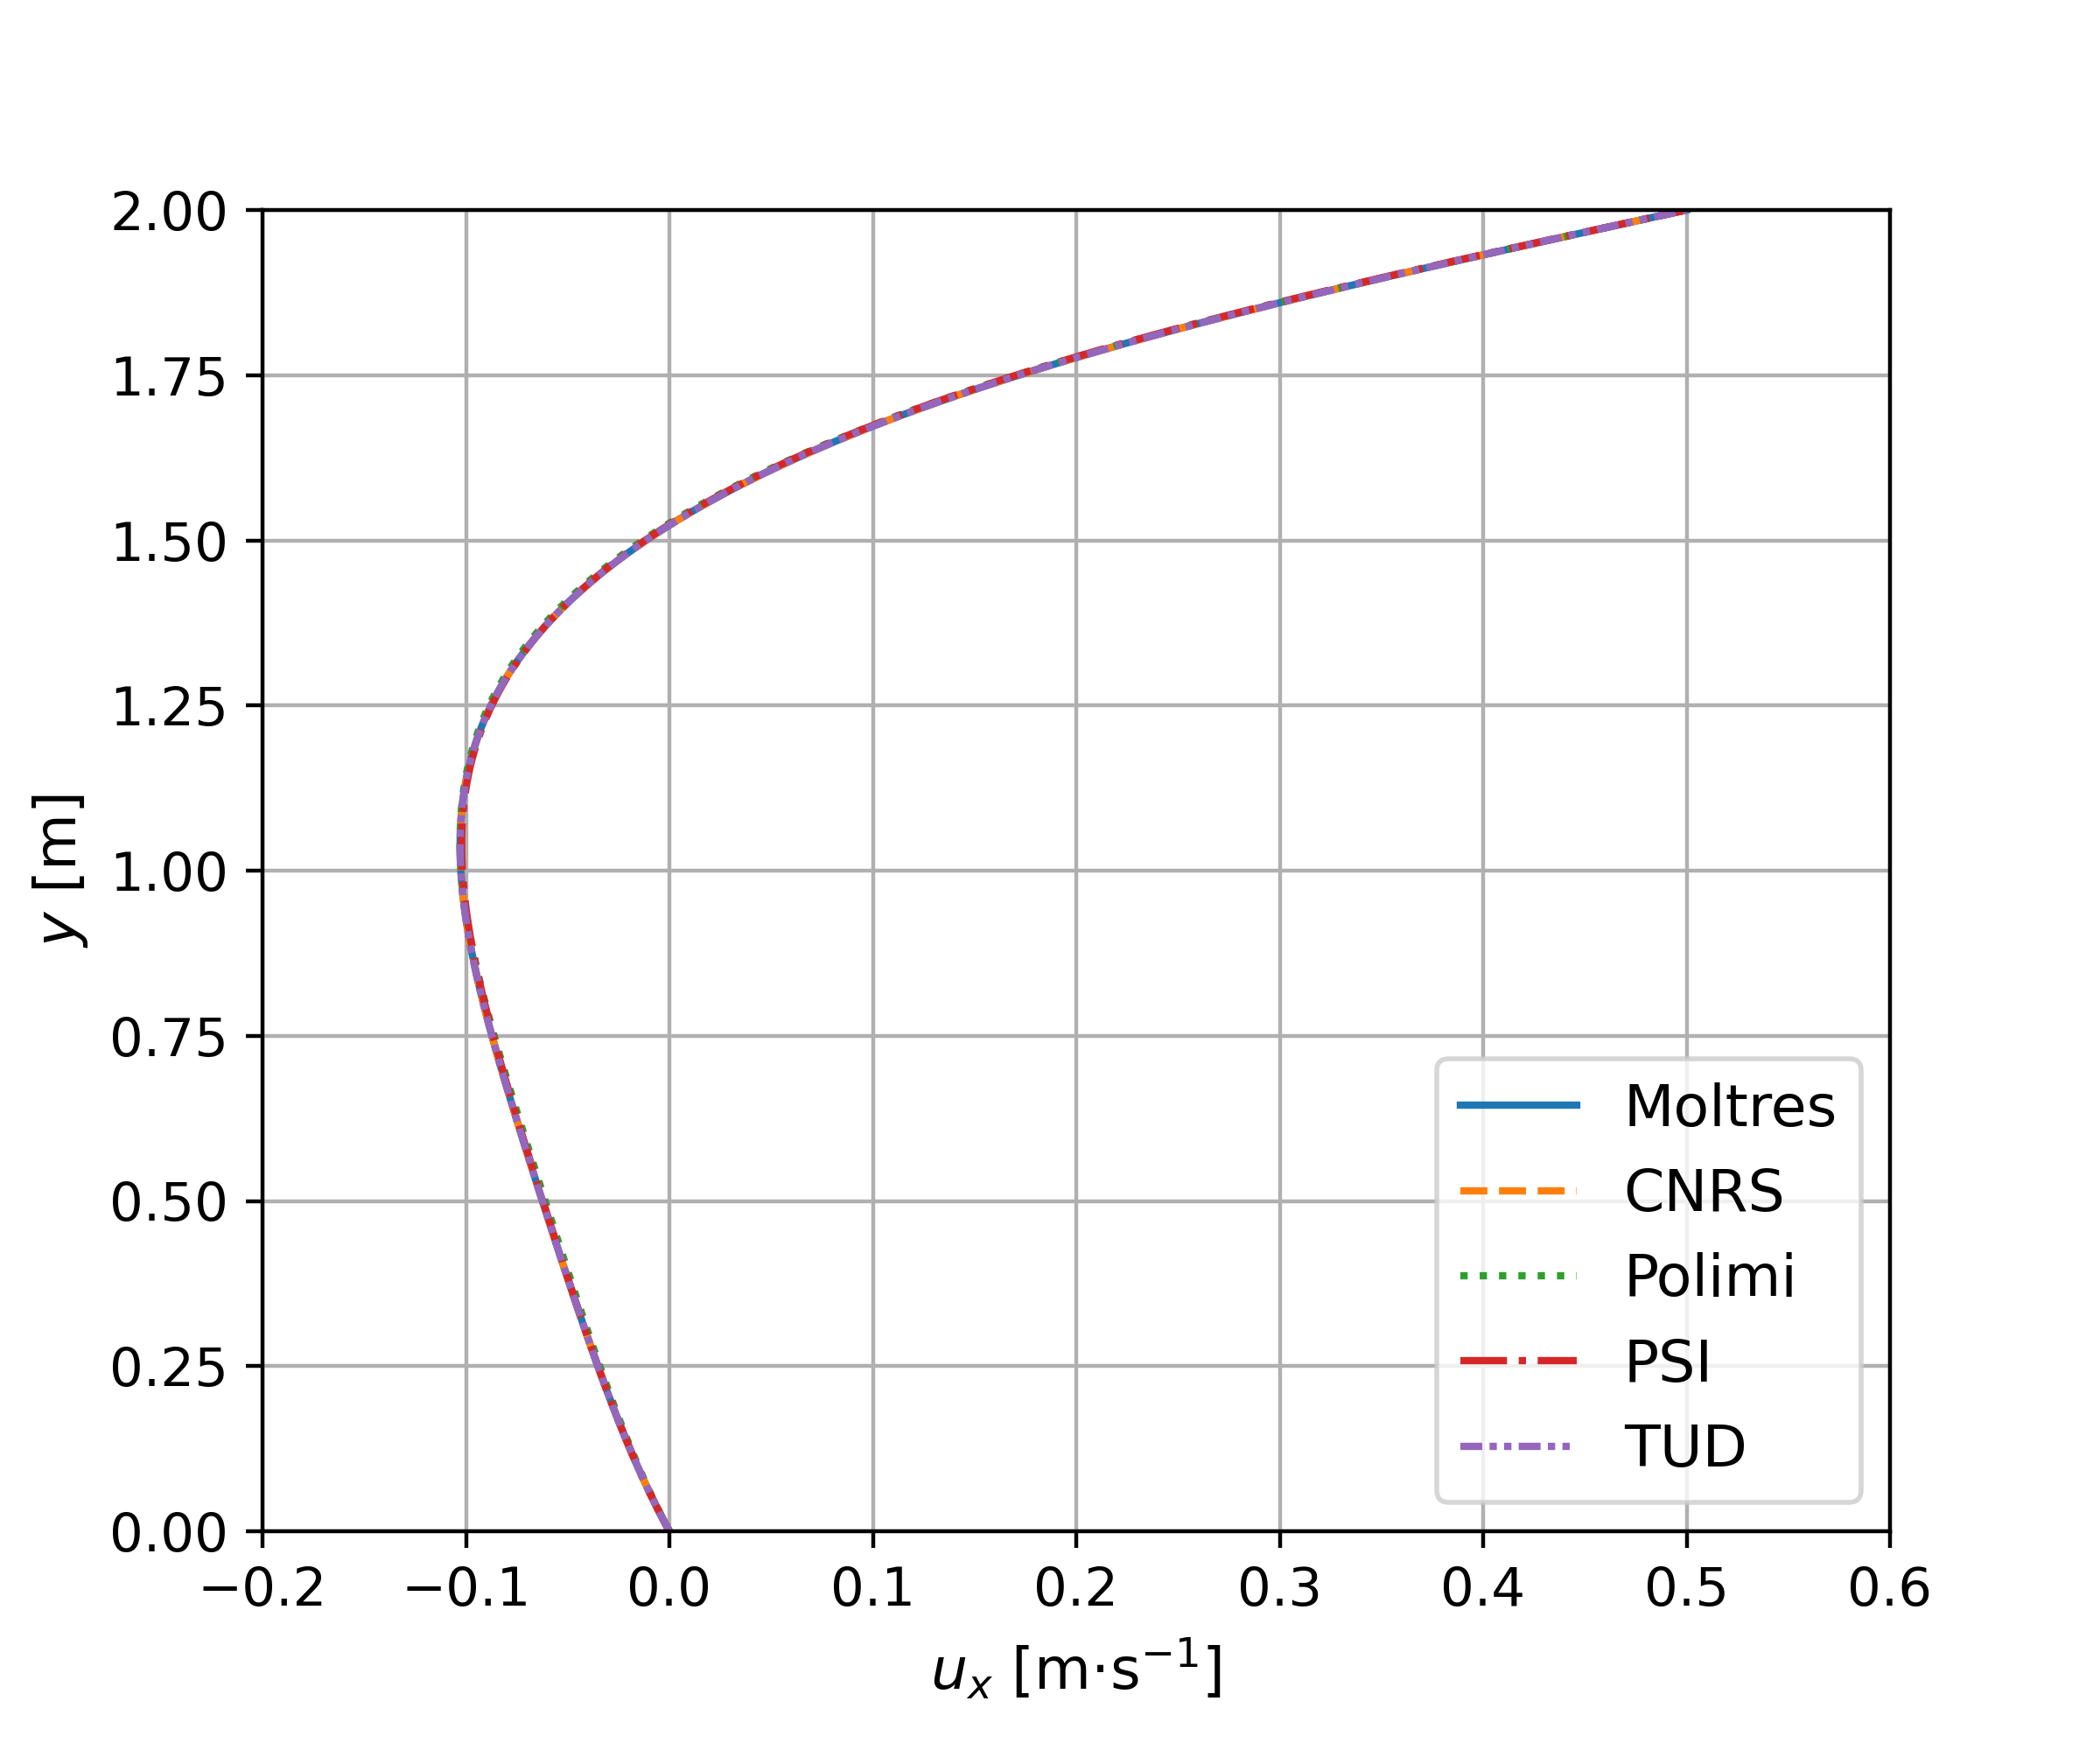
\includegraphics[width=.8\columnwidth]{0-1-vel-plot}
	\caption{Step 0.1 - Horizontal velocity component along BB'.}
	\label{fig:0.1}
\end{figure}
%
\begin{figure}[tb]
	\centering
	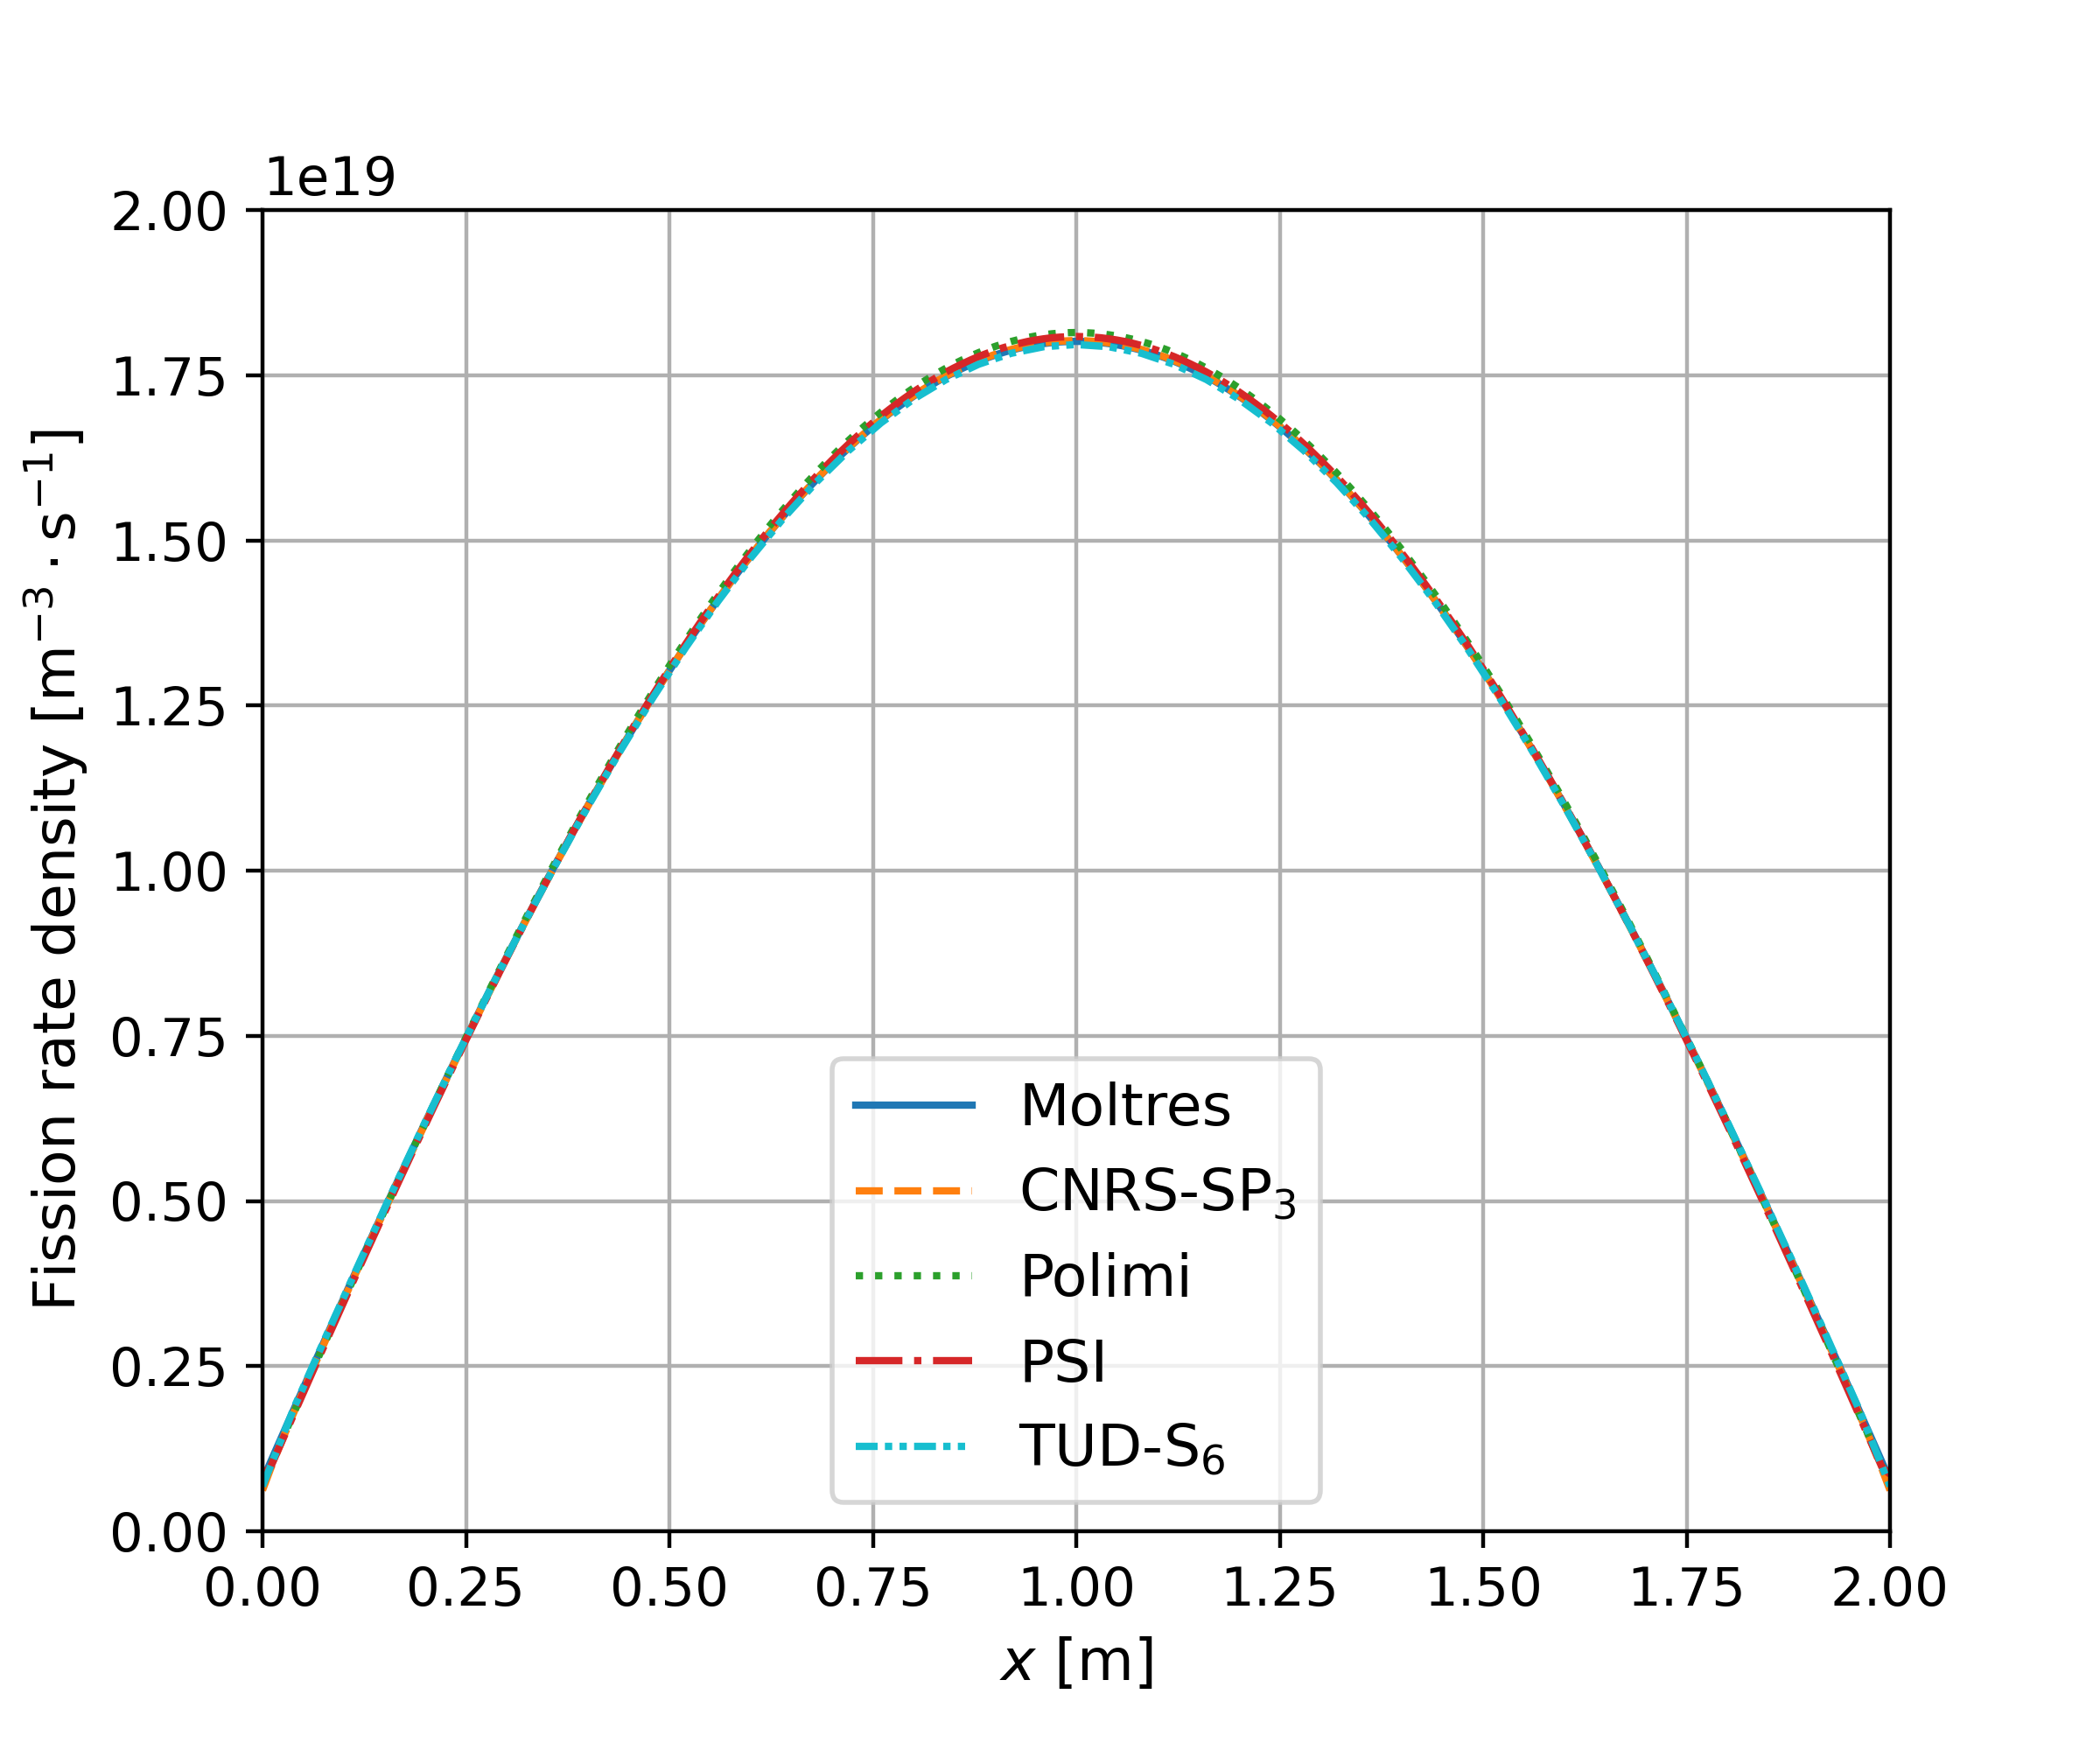
\includegraphics[width=.8\columnwidth]{0-2-fiss-plot}
	\caption{Step 0.2 - Fission rate density along AA'.}
	\label{fig:0.2}
\end{figure}
%
\begin{figure}[tb]
	\centering
	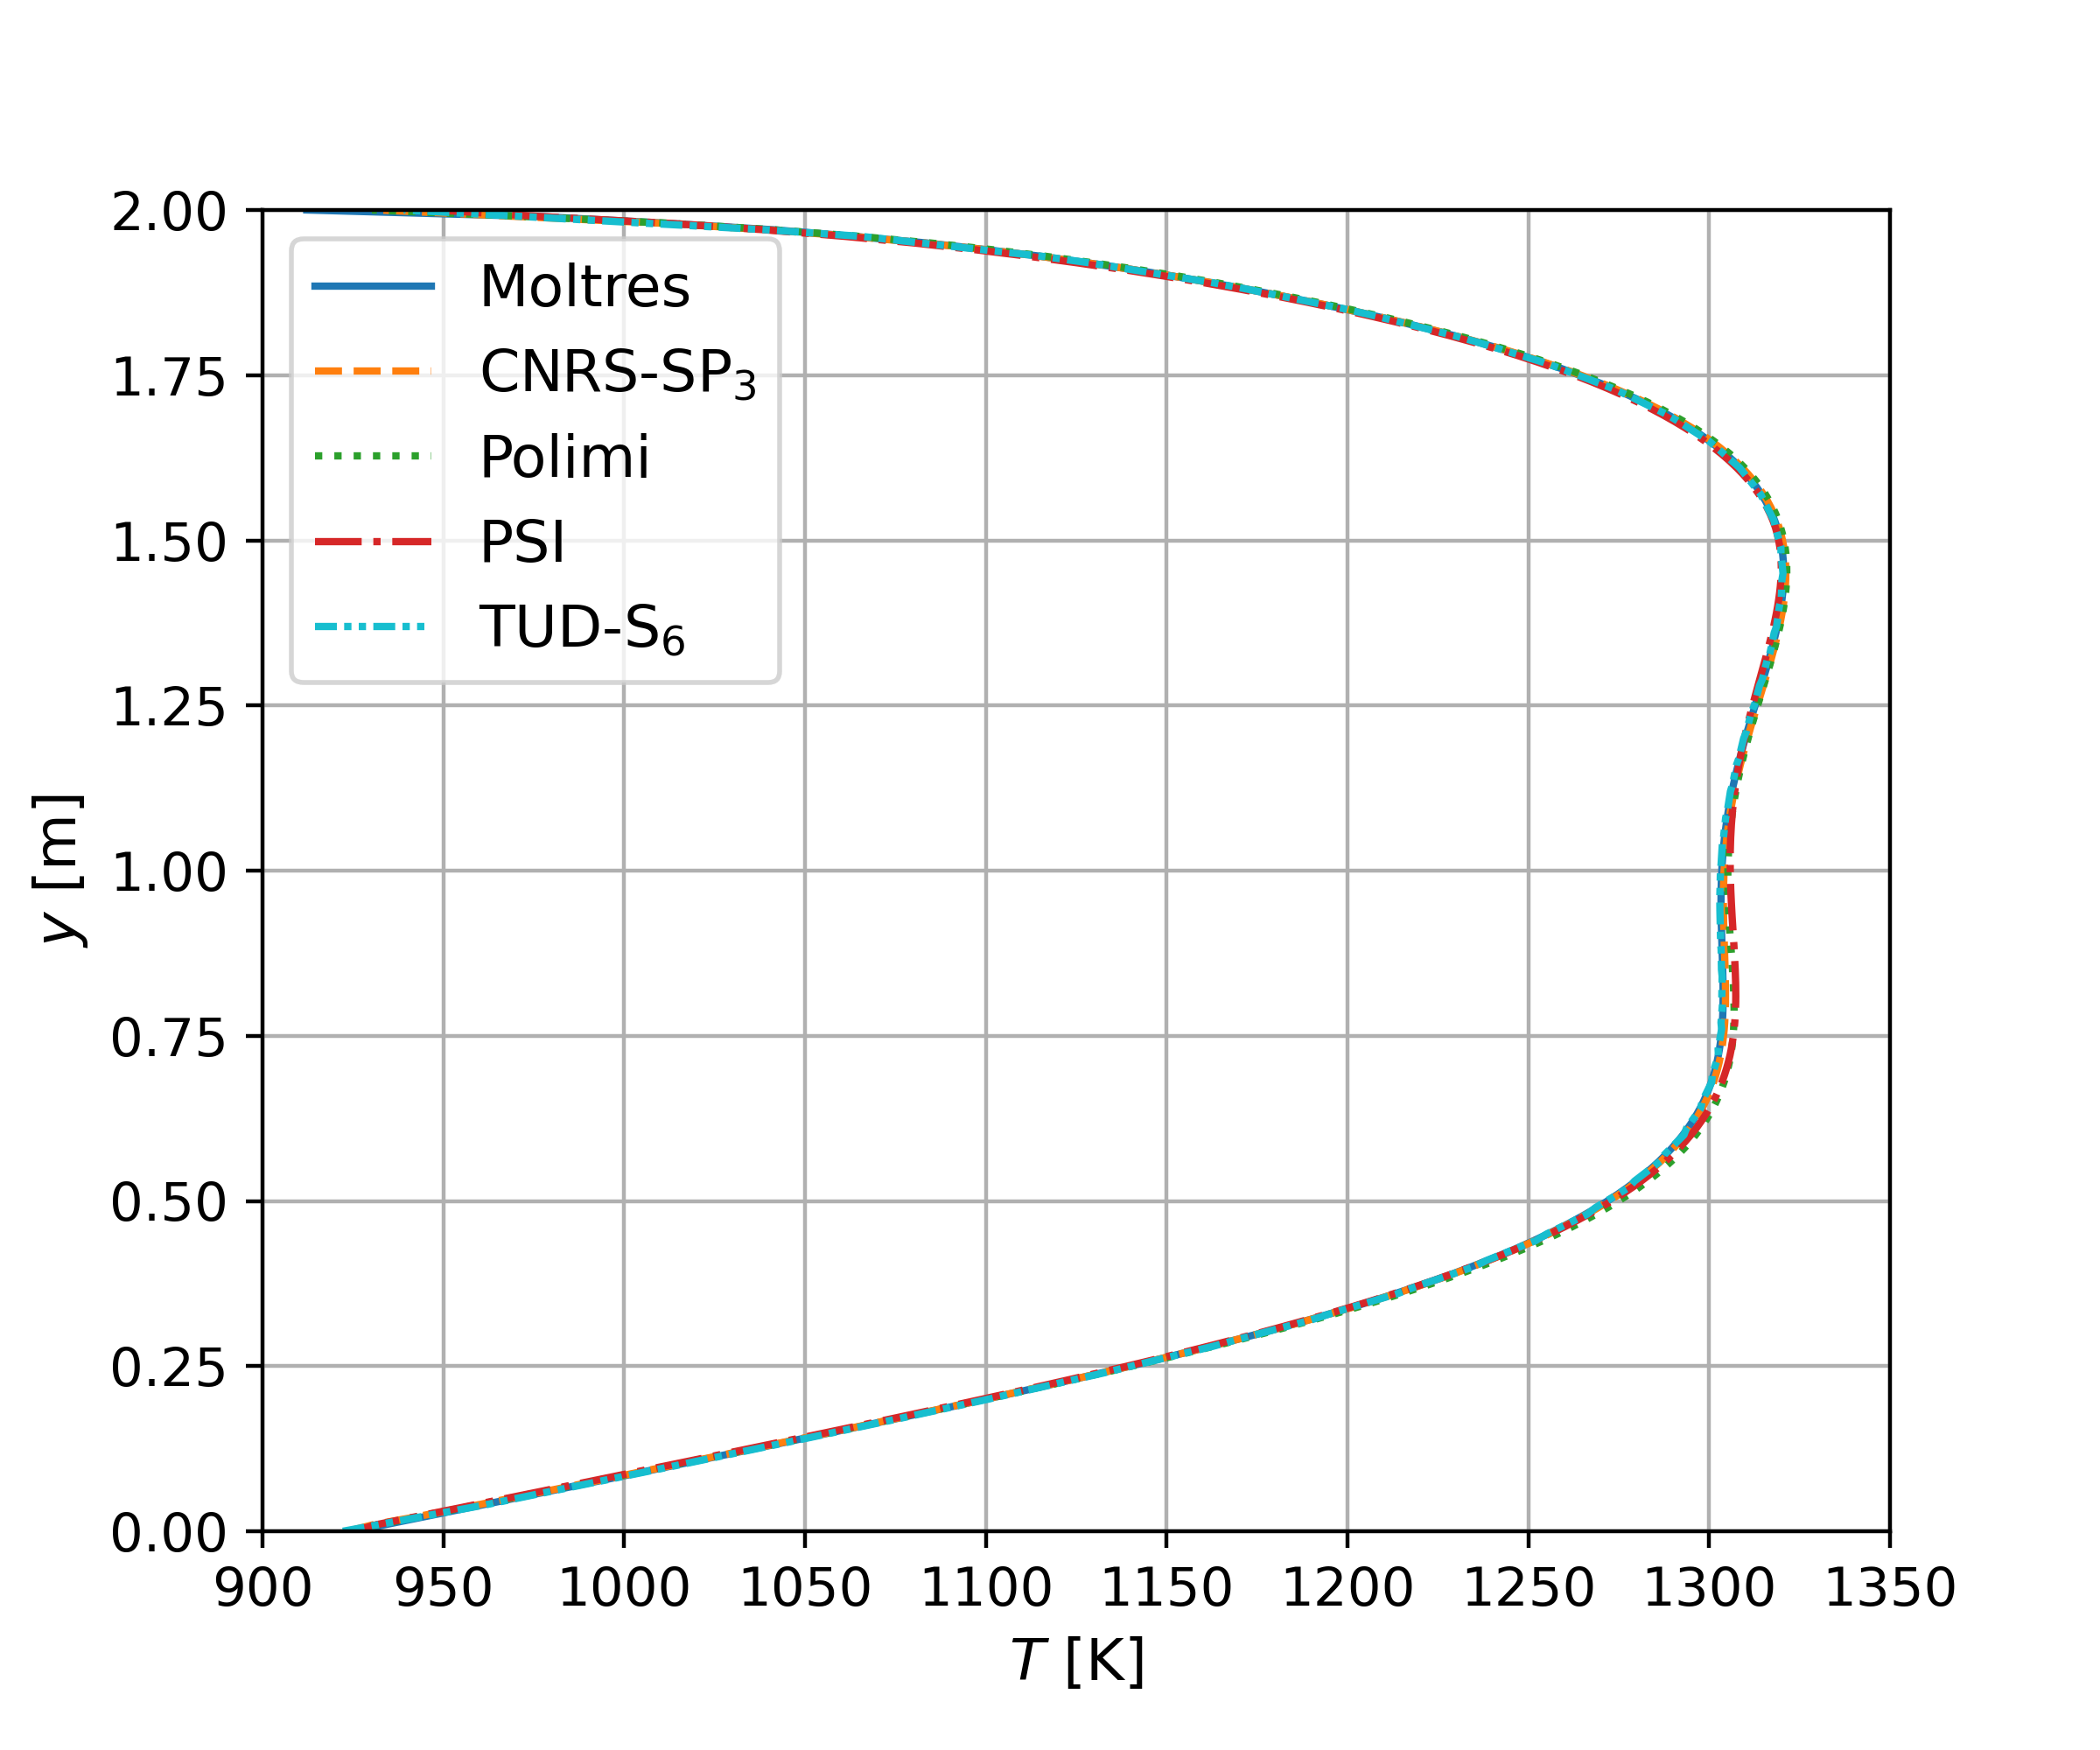
\includegraphics[width=.8\columnwidth]{0-3-temp-plot}
	\caption{Step 0.3 - Temperature distribution along BB'.}
	\label{fig:0.3}
\end{figure}
%
\begin{table}[tb]
	\caption{Discrepancy values for the results from Phase 0.}
	\centering
	\footnotesize
	\setlength\tabcolsep{2pt}
	\begin{tabular}{l l c S S}
		\toprule
		\multirow{2}{*}{\textbf{Step}} & \multirow{2}{*}{\textbf{Observable}} & \multirow{2}{*}{\textbf{Centerline}} & \multicolumn{2}{c}{\textbf{Discrepancies [\%]}} \\
		& & & {Moltres} & {Benchmark} \\
		\midrule
		\multirow{4}{*}{0.1} &
		\multirow{2}{*}{$u_x$ [m$\cdot$s$^{-1}$]} & AA' & 0.247 & 0.253 \\
		& & BB' & 0.266 & 0.318 \\
		\cmidrule{2-5}
		& \multirow{2}{*}{$u_y$ [m$\cdot$s$^{-1}$]} & AA' & 0.540 & 0.598
		\\
		& & BB' & 0.468 & 0.795 \\
		\midrule
		{0.2} &
		{$\sum^G_i \Sigma_{f,i} \phi_i(\vec{r})$
		[m$^{-3}\cdot$s$^{-1}$]} & AA' & 0.313 & 0.285 \\
		\midrule
		\multirow{2}{*}{0.3} &
		\multirow{2}{*}{$T$ [K]} & AA' & 0.090 & 0.085 \\
		& & BB' & 0.164 & 0.083 \\
		\bottomrule
	\end{tabular}
	\label{table:disc0}
\end{table}

Figures \ref{fig:0.1}, \ref{fig:0.2}, and \ref{fig:0.3} show that Moltres
accurately reproduced all three sets of results in Phase 0 for the velocity
field, fission rate density, and temperature, respectively.
Table \ref{table:disc0} reports the discrepancy values from Moltres for Phase 0
and the corresponding average discrepancy values from the benchmark
\citep{tiberga_results_2020}. Moltres performs excellently as all discrepancy
values are on the same order of magnitude as those from the benchmark,
except the discrepancy value for $T$ along centerline BB' which is marginally
higher at 0.164\% compared to 0.083\% from the benchmark average. However, we
note in Figure \ref{fig:0.3} that the $T$ distribution from Moltres is almost
identical to the corresponding distributions from CNRS-$SP_3$ and TUD-$S_6$.

Table \ref{table:temp} shows the temperature values from Moltres and the
benchmark at nine equidistant points along centerlines AA' and BB'. Similar to
Figure \ref{fig:0.3}, most temperature values from Moltres fall within the
corresponding range of values from the benchmark with the exception of the
value at the coordinates (1, 2); Moltres underpredicts the temperature at 912.3
K compared to the benchmark values which range between 930.3 K
and 948.1 K. This point on the top boundary lies directly
downstream of
the velocity boundary condition discontinuity at the top-left corner.
In general, corner singularities are generally difficult to approximate with
Galerkin methods \citep{kuhlmann_lid-driven_2018}.
The \gls{SUPG} stabilization scheme dampens numerical oscillations by
introducing pointwise artificial thermal diffusivity which depends strongly on
the inverse of local velocity magnitude \citep{peterson_overview_2018}.
Therefore, while the \gls{SUPG} scheme was very effective in eliminating
spurious numerical oscillations everywhere else, it provides little damping
along the top boundary due to the relatively large non-zero velocity boundary
condition. On the other hand, the temperature values in the rest of the domain
and the average discrepancies of the other variables show that Moltres can
still accurately reproduce the expected results and the temperature deviations
along the top boundary do not impact the overall integrity of our results.

\begin{table*}[tb]
	\caption{Temperature distribution along centerlines $AA'$ and $BB'$.}
	\centering
	\footnotesize
	\setlength\tabcolsep{1.5pt}
%	\hspace*{-2cm}
	\begin{tabular}{c c c c c c c c c c c}
		\toprule
		\multirow{2}{*}{\textbf{Observable}} & \multirow{2}{*}{\textbf{Code}} & \multicolumn{9}{c}{\textbf{Results along $AA'$} (point coordinates are expressed in m)} \\
		& & {(0,1)} & {(0.25,1)} & {(0.5,1)} & {(0.75,1)} & {(1,1)} & {(1.25,1)} & {(1.5,1)} & {(1.75,1)} & {(2,1)} \\
		\midrule
		\multirow{7}{*}{$T$ [K]} & Moltres & 9.251E+02 & 1.194E+03 & 1.357E+03 & 1.361E+03 &
		1.303E+03 & 1.224E+03 & 1.131E+03 & 1.035E+03 & 9.251E+02 \\
		& CNRS-$SP_1$ & 9.253E+02 & 1.194E+03 & 1.358E+03 & 1.363E+03 & 1.305E+03 & 1.224E+03 & 1.131E+03 & 1.034E+03 & 9.251E+02 \\
		& CNRS-$SP_3$ & 9.236E+02 & 1.194E+03 & 1.357E+03 & 1.361E+03 & 1.304E+03 & 1.224E+03 & 1.131E+03 & 1.034E+03 & 9.235E+02 \\
		& Polimi & 9.253E+02 & 1.196E+03 & 1.361E+03 & 1.364E+03 & 1.305E+03 & 1.224E+03 & 1.132E+03 & 1.035E+03 & 9.252E+02 \\
		& PSI & 9.253E+02 & 1.196E+03 & 1.356E+03 & 1.363E+03 & 1.306E+03 & 1.226E+03 & 1.133E+03 & 1.037E+03 & 9.252E+02 \\
		& TUD-$S_2$ & 9.212E+02 & 1.194E+03 & 1.359E+03 & 1.364E+03 & 1.305E+03 & 1.224E+03 & 1.131E+03 & 1.032E+03 & 9.225E+02 \\
		& TUD-$S_6$ & 9.219E+02 & 1.194E+03 & 1.356E+03 & 1.360E+03 & 1.303E+03 & 1.223E+03 & 1.131E+03 & 1.034E+03 & 9.233E+02 \\
		\midrule
		\midrule
		\multirow{2}{*}{\textbf{Observable}} & \multirow{2}{*}{\textbf{Code}} & \multicolumn{9}{c}{\textbf{Results along $BB'$} (point coordinates are expressed in m)} \\
		& & {(1,0)} & {(1,0.25)} & {(1,0.5)} & {(1,0.75)} & {(1,1)} & {(1,1.25)} & {(1,1.5)} & {(1,1.75)} & {(1,2)} \\
		\midrule
		\multirow{7}{*}{$T$ [K]} & Moltres & 9.251E+02 & 1.140E+03 & 1.272E+03 & 1.303E+03 &
		1.303E+03 & 1.313E+03 & 1.320E+03 & 1.264E+03 & 9.123E+02 \\
		& CNRS-$SP_1$ & 9.252E+02 & 1.139E+03 & 1.273E+03 & 1.305E+03 & 1.305E+03 & 1.314E+03 & 1.321E+03 & 1.265E+03 & 9.322E+02 \\
		& CNRS-$SP_3$ & 9.236E+02 & 1.140E+03 & 1.272E+03 & 1.304E+03 & 1.304E+03 & 1.313E+03 & 1.320E+03 & 1.265E+03 & 9.322E+02 \\
		& Polimi & 9.253E+02 & 1.140E+03 & 1.275E+03 & 1.307E+03 & 1.305E+03 & 1.313E+03 & 1.321E+03 & 1.265E+03 & 9.303E+02 \\
		& PSI & 9.252E+02 & 1.139E+03 & 1.273E+03 & 1.307E+03 & 1.306E+03 & 1.312E+03 & 1.319E+03 & 1.263E+03 & 9.481E+02 \\
		& TUD-$S_2$ & 9.215E+02 & 1.139E+03 & 1.273E+03 & 1.305E+03 & 1.305E+03 & 1.315E+03 & 1.322E+03 & 1.265E+03 & 9.374E+02 \\
		& TUD-$S_6$ & 9.222E+02 & 1.140E+03 & 1.272E+03 & 1.303E+03 & 1.303E+03 & 1.312E+03 & 1.319E+03 & 1.264E+03 & 9.390E+02 \\
		\bottomrule
	\end{tabular}
	\label{table:temp}
\end{table*}
%
\begin{table}[tb]
    \caption{Reactivity $\rho$ and change in reactivity
    $\left(\rho_a - \rho_b\right)$ values from Steps 0.2, 1.1,
    1.2, and 1.3. All units are in pcm.}
    \centering
    \footnotesize
    \setlength\tabcolsep{2pt}
    \begin{tabular}{l S S S S}
        \toprule
        \multirow{2}{*}{\textbf{Software}} & {\textbf{Step 0.2}} &
        {\textbf{Step 1.1}} & {\textbf{Step 1.2}} & {\textbf{Step 1.3}} \\
        & {$\rho_{s_{0.2}}$}
        & {$\rho_{s_{1.1}} - \rho_{s_{0.2}}$}
        & {$\rho_{s_{1.2}} - \rho_{s_{1.1}}$}
        & {$\rho_{s_{1.3}} - \rho_{s_{0.2}}$} \\
        \midrule
        Moltres     & 465.6 & -62.7 & -1142.2 & -1207.7 \\
        CNRS-$SP_1$ & 411.3 & -62.5 & -1152.0 & -1220.5 \\
        CNRS-$SP_3$ & 353.7 & -62.6 & -1152.7 & -1220.7 \\
        Polimi      & 421.2 & -62.0 & -1161.0 & -1227.0 \\
        PSI         & 411.7 & -63.0 & -1154.8 & -1219.6 \\
        TUD-$S_2$   & 482.6 & -62.0 & -1145.2 & -1208.5 \\
        TUD-$S_6$   & 578.1 & -60.7 & -1122.0 & -1184.4 \\
        \bottomrule
    \end{tabular}
    \label{table:rho}
\end{table}

Lastly, we observe in table \ref{table:rho} that the reactivity $\rho$ value of
465.6 pcm from Moltres falls well within the range of $\rho$ values from the
benchmark which range from 353.7 pcm up to 578.1 pcm. Moltres' $\rho$ value
agrees closest to the results from the
software packages, namely CNRS-$SP_1$, Polimi, PSI, and TUD-$S_2$, which adopt
the neutron diffusion model or theoretically-equivalent models such as $SP_1$
and $S_2$ neutron transport models).

\subsection{Phase 1 results \& discussion}

Table \ref{table:disc1} shows the discrepancy values from Moltres for Steps
1.1, 1.2, and 1.3,
and the corresponding average discrepancy values from the benchmark
\citep{tiberga_results_2020}. The subsequent subsections discuss the results
for each benchmark step.

\subsubsection{Step 1.1: Circulating fuel}
%
\begin{figure*}[tb]
	\centering
    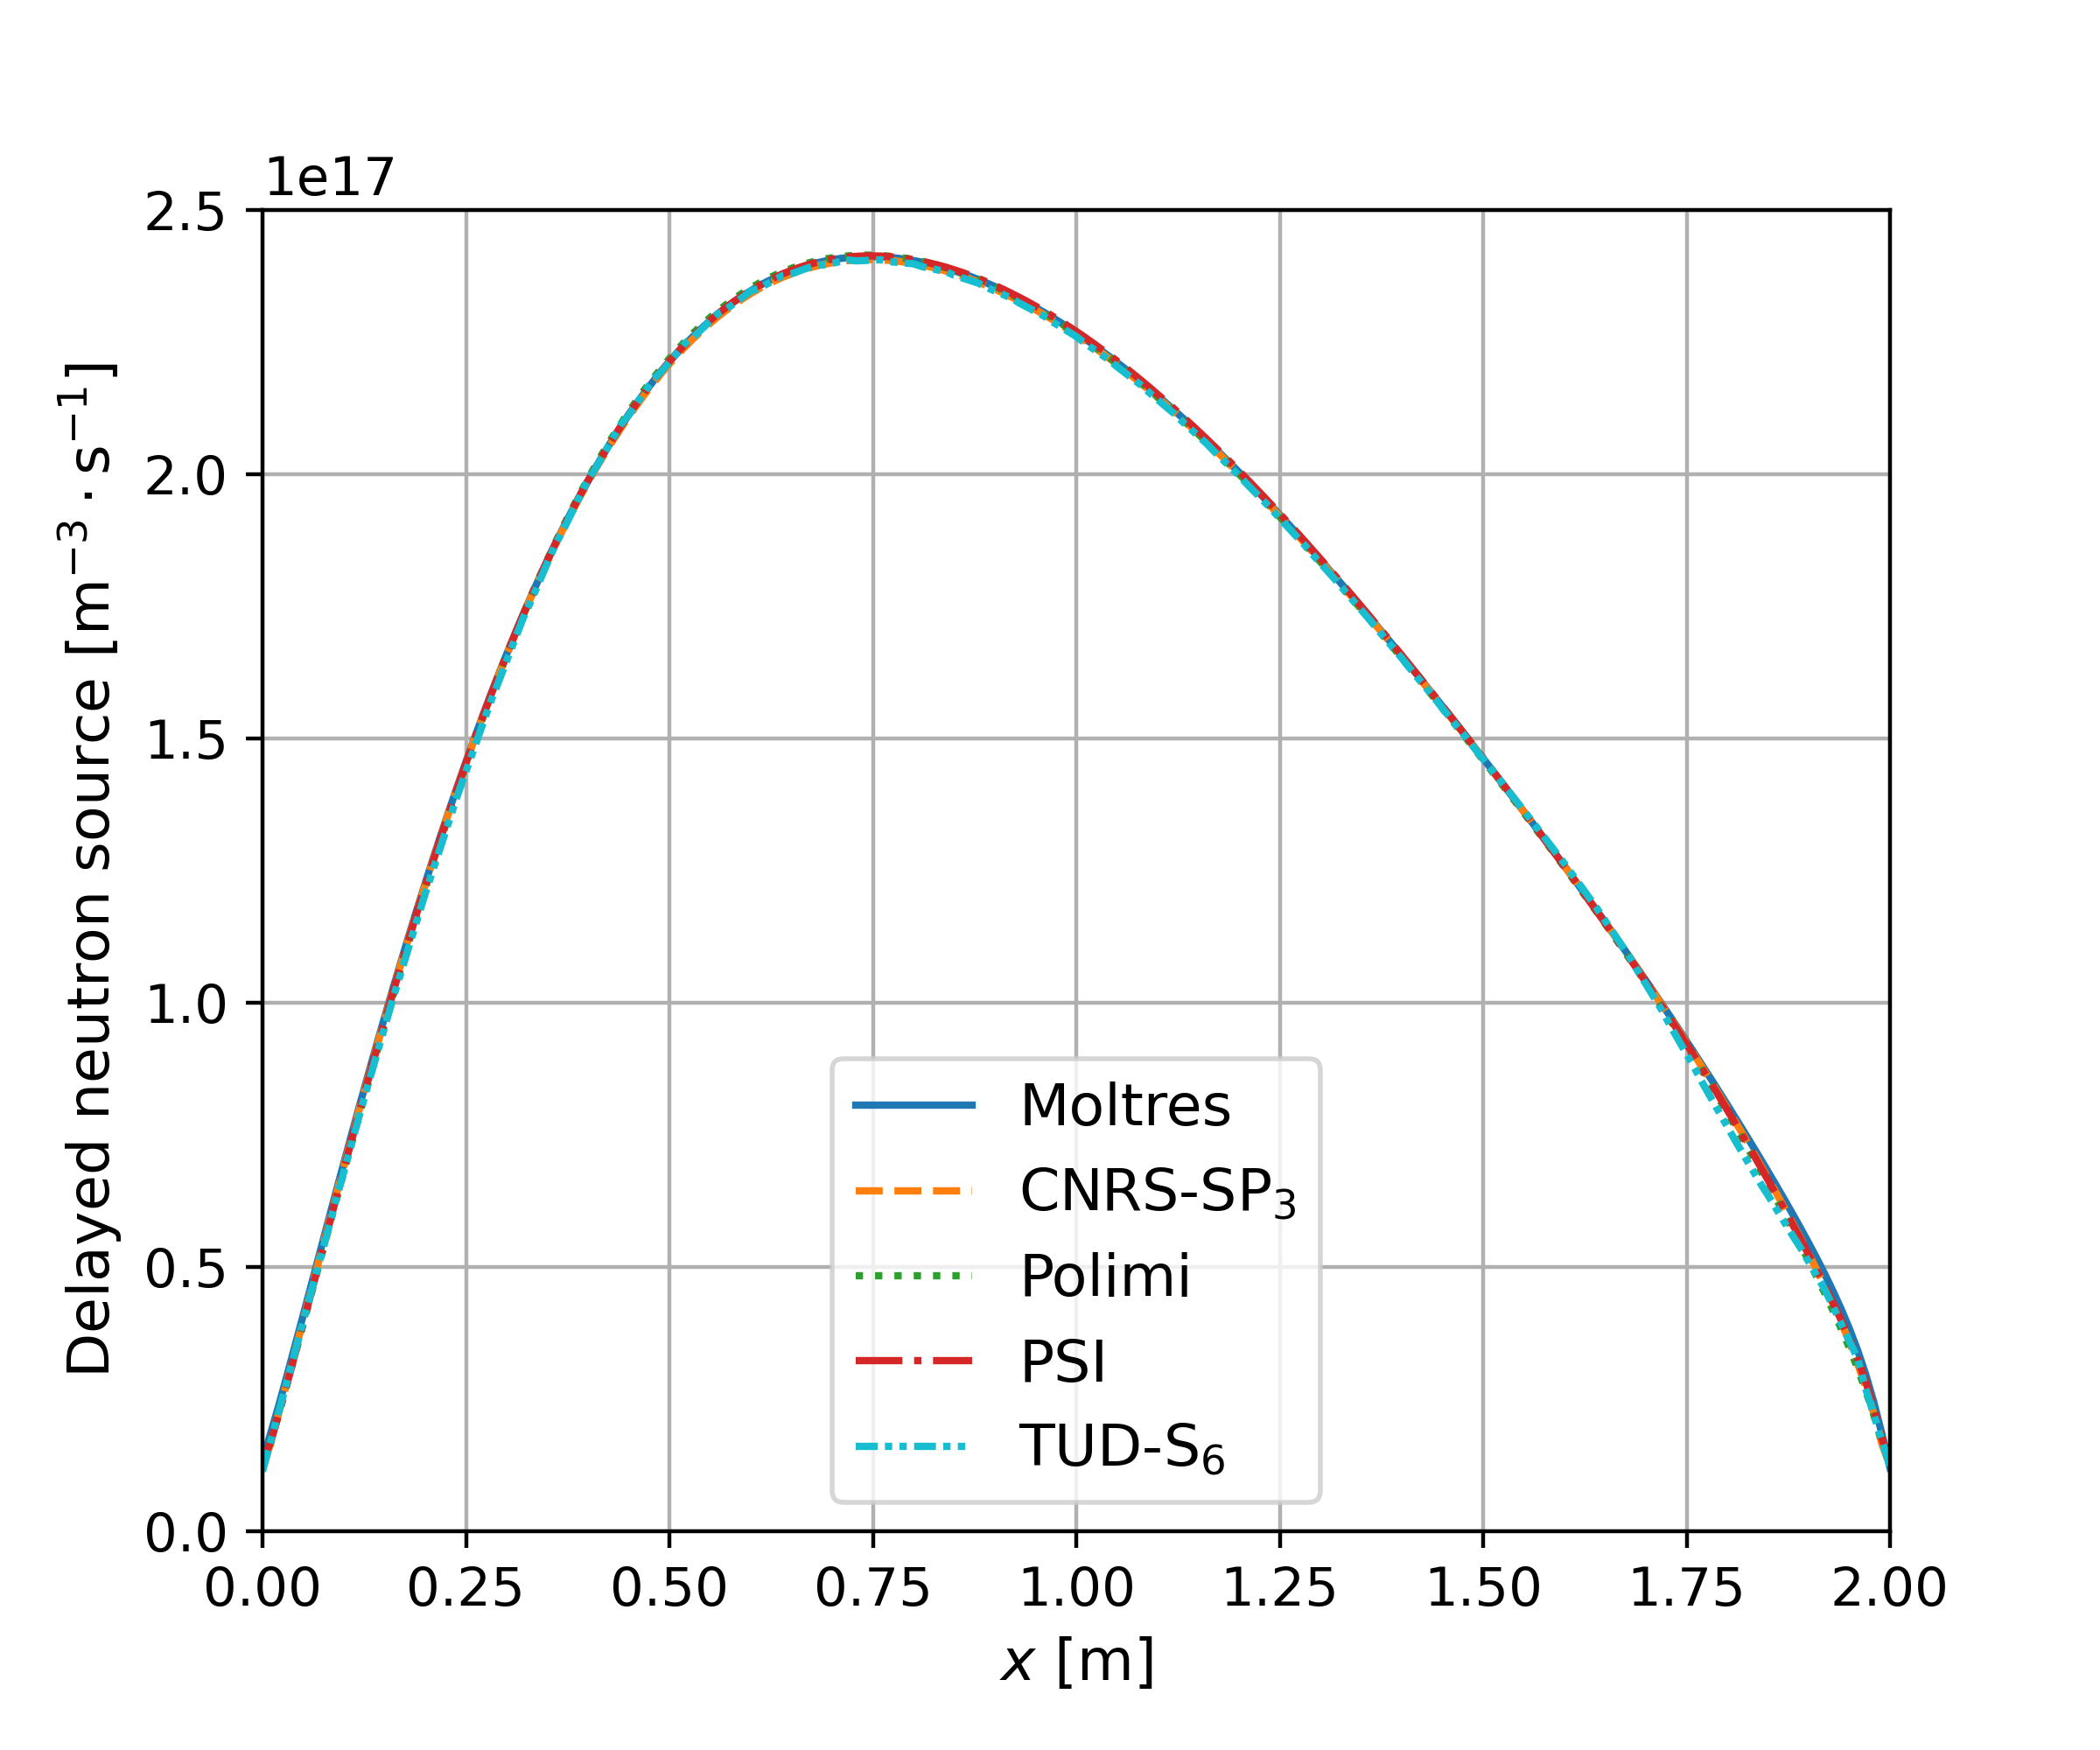
\includegraphics[width=.8\columnwidth]{1-1-dnp-x-plot}
    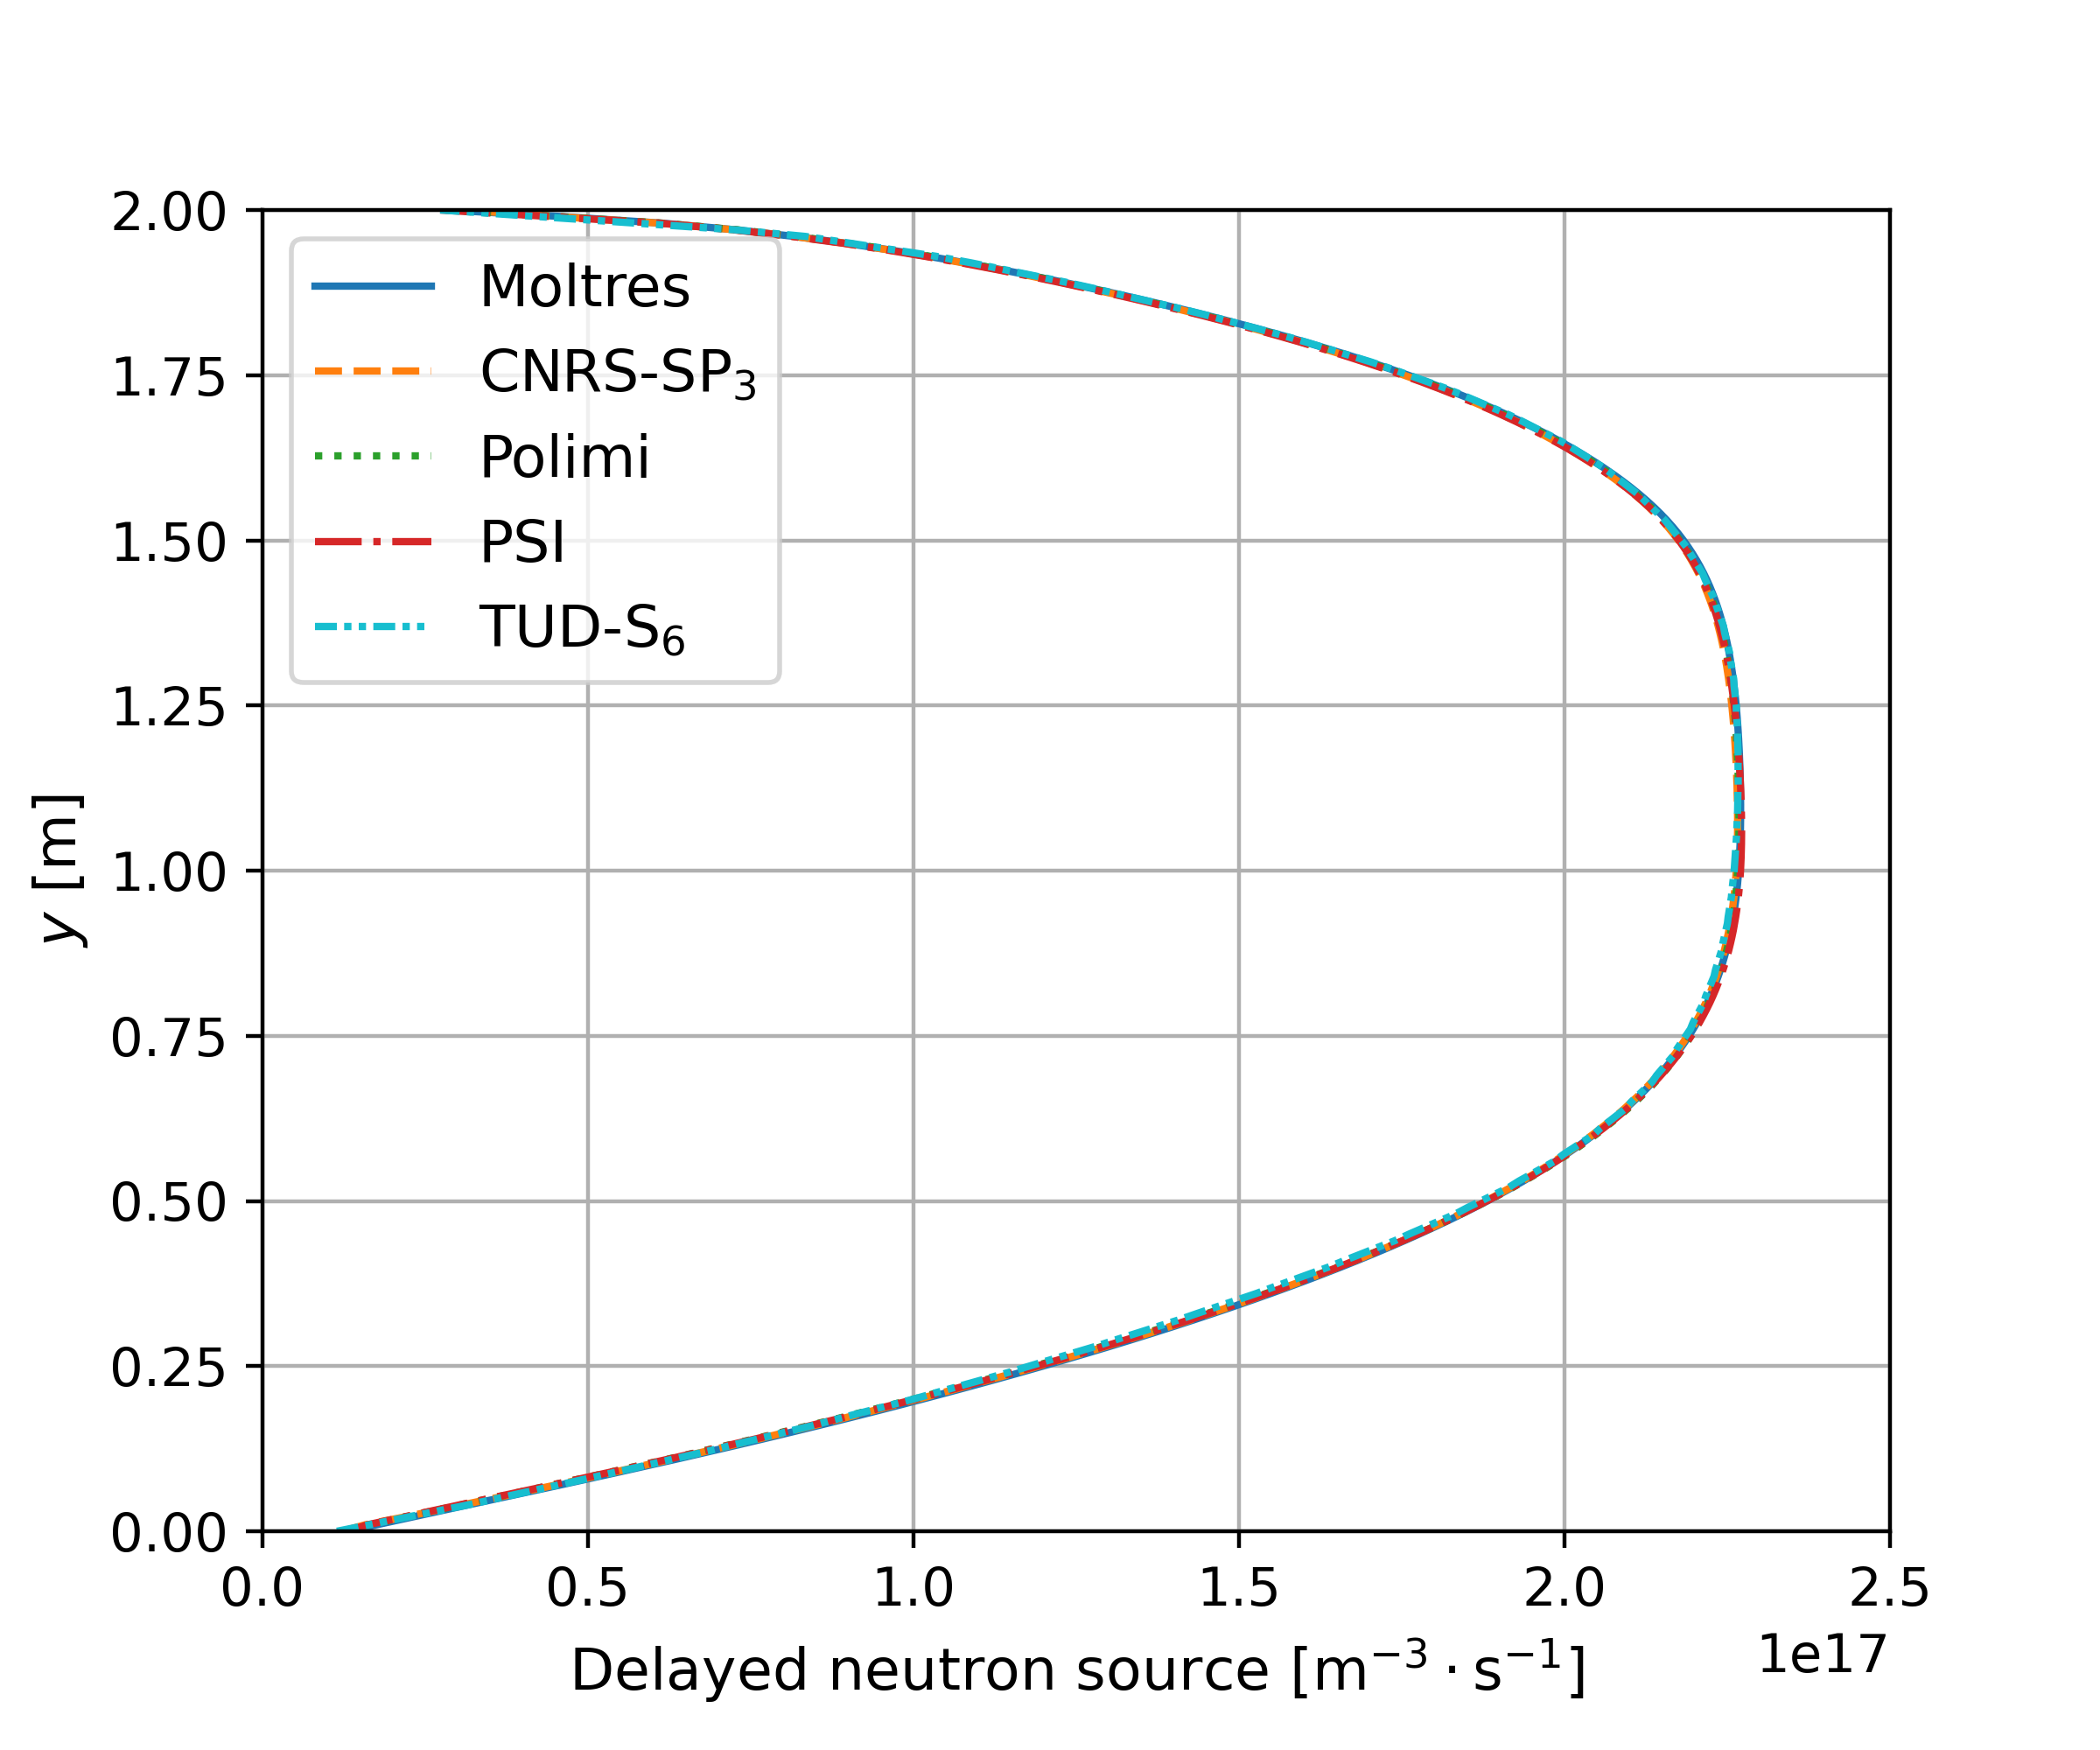
\includegraphics[width=.8\columnwidth]{1-1-dnp-y-plot}
	\caption{Step 1.1 - Delayed neutron source along AA' and BB'.}
	\label{fig:1.1}
\end{figure*}

Figure \ref{fig:1.1} shows the delayed neutron source distribution along BB'.
Moltres produces similar results to the benchmark average as the
discrepancies in the delayed neutron source along both centerlines in Table
\ref{table:disc1} are on
the same order of magnitude. We also note that approximating the delayed
neutron precursor concentrations with the zeroth-order discontinuous finite
element method does not impact the overall accuracy because it is
similar to first-order finite volume methods which also use constant test
functions.
In Table \ref{table:rho}, we observe that the change in
$\rho$ relative to Step 0.2 is $-62.7$ pcm for Moltres and this value is
consistent with the $-63$ to $-62$ pcm range that most of the benchmark values
fall in.
%
\begin{table*}[tb]
	\caption{Discrepancy values for the results from Phase 1.}
	\centering
	\footnotesize
	\begin{tabular}{l l c S S}
		\toprule
		\multirow{2}{*}{\textbf{Step}} & \multirow{2}{*}{\textbf{Observable}} & \multirow{2}{*}{\textbf{Centerline}} & \multicolumn{2}{c}{\textbf{Discrepancies [\%]}} \\
		& & & {Moltres} & {Benchmark} \\
		\midrule
		\multirow{2}{*}{1.1} &
		\multirow{2}{*}{$\sum_j \lambda_j C_j$ [m$^{-3}\cdot$s$^{-1}$]} & AA' & 0.603 & 0.346 \\
		& & BB' & 0.327 & 0.294 \\
		\midrule
		\multirow{4}{*}{1.2} &
		\multirow{2}{*}{$T$ [K]} & AA' & 0.076 & 0.095 \\
		& & BB' & 0.179 & 0.089 \\
		\cmidrule{2-5}
		& \multirow{2}{*}{\footnotesize $\Delta\left[\sum^G_i \Sigma_{f,i} \phi_i(\vec{r})
		\right]_{s_{1.2}-s_{0.2}}$ [m$^{-3}\cdot$s$^{-1}$]} & AA' & 1.110 & 1.576 \\
		& & BB' & 1.089 & 1.133 \\
		\midrule
		\multirow{7}{*}{1.3} &
		{$u_x$ [m$\cdot$s$^{-1}$]} & AA' & 0.123 & 0.691 \\
		\cmidrule{2-5}
		& \multirow{2}{*}{$u_y$ [m$\cdot$s$^{-1}$]} & AA' & 0.237 & 0.329 \\
		& & BB' & 0.238 & 0.356 \\
		\cmidrule{2-5}
		& \multirow{2}{*}{$T$ [K]} & AA' & 0.064 & 0.057 \\
		& & BB' & 0.070 & 0.080 \\
		\cmidrule{2-5}
		& \multirow{2}{*}{$\sum_j \lambda_j C_j$ [m$^{-3}\cdot$s$^{-1}$]} & AA' & 1.043 & 0.460 \\
		& & BB' & 0.462 & 1.194 \\
		\bottomrule
	\end{tabular}
	\label{table:disc1}
\end{table*}
%
\begin{figure*}[tb]
	\centering
	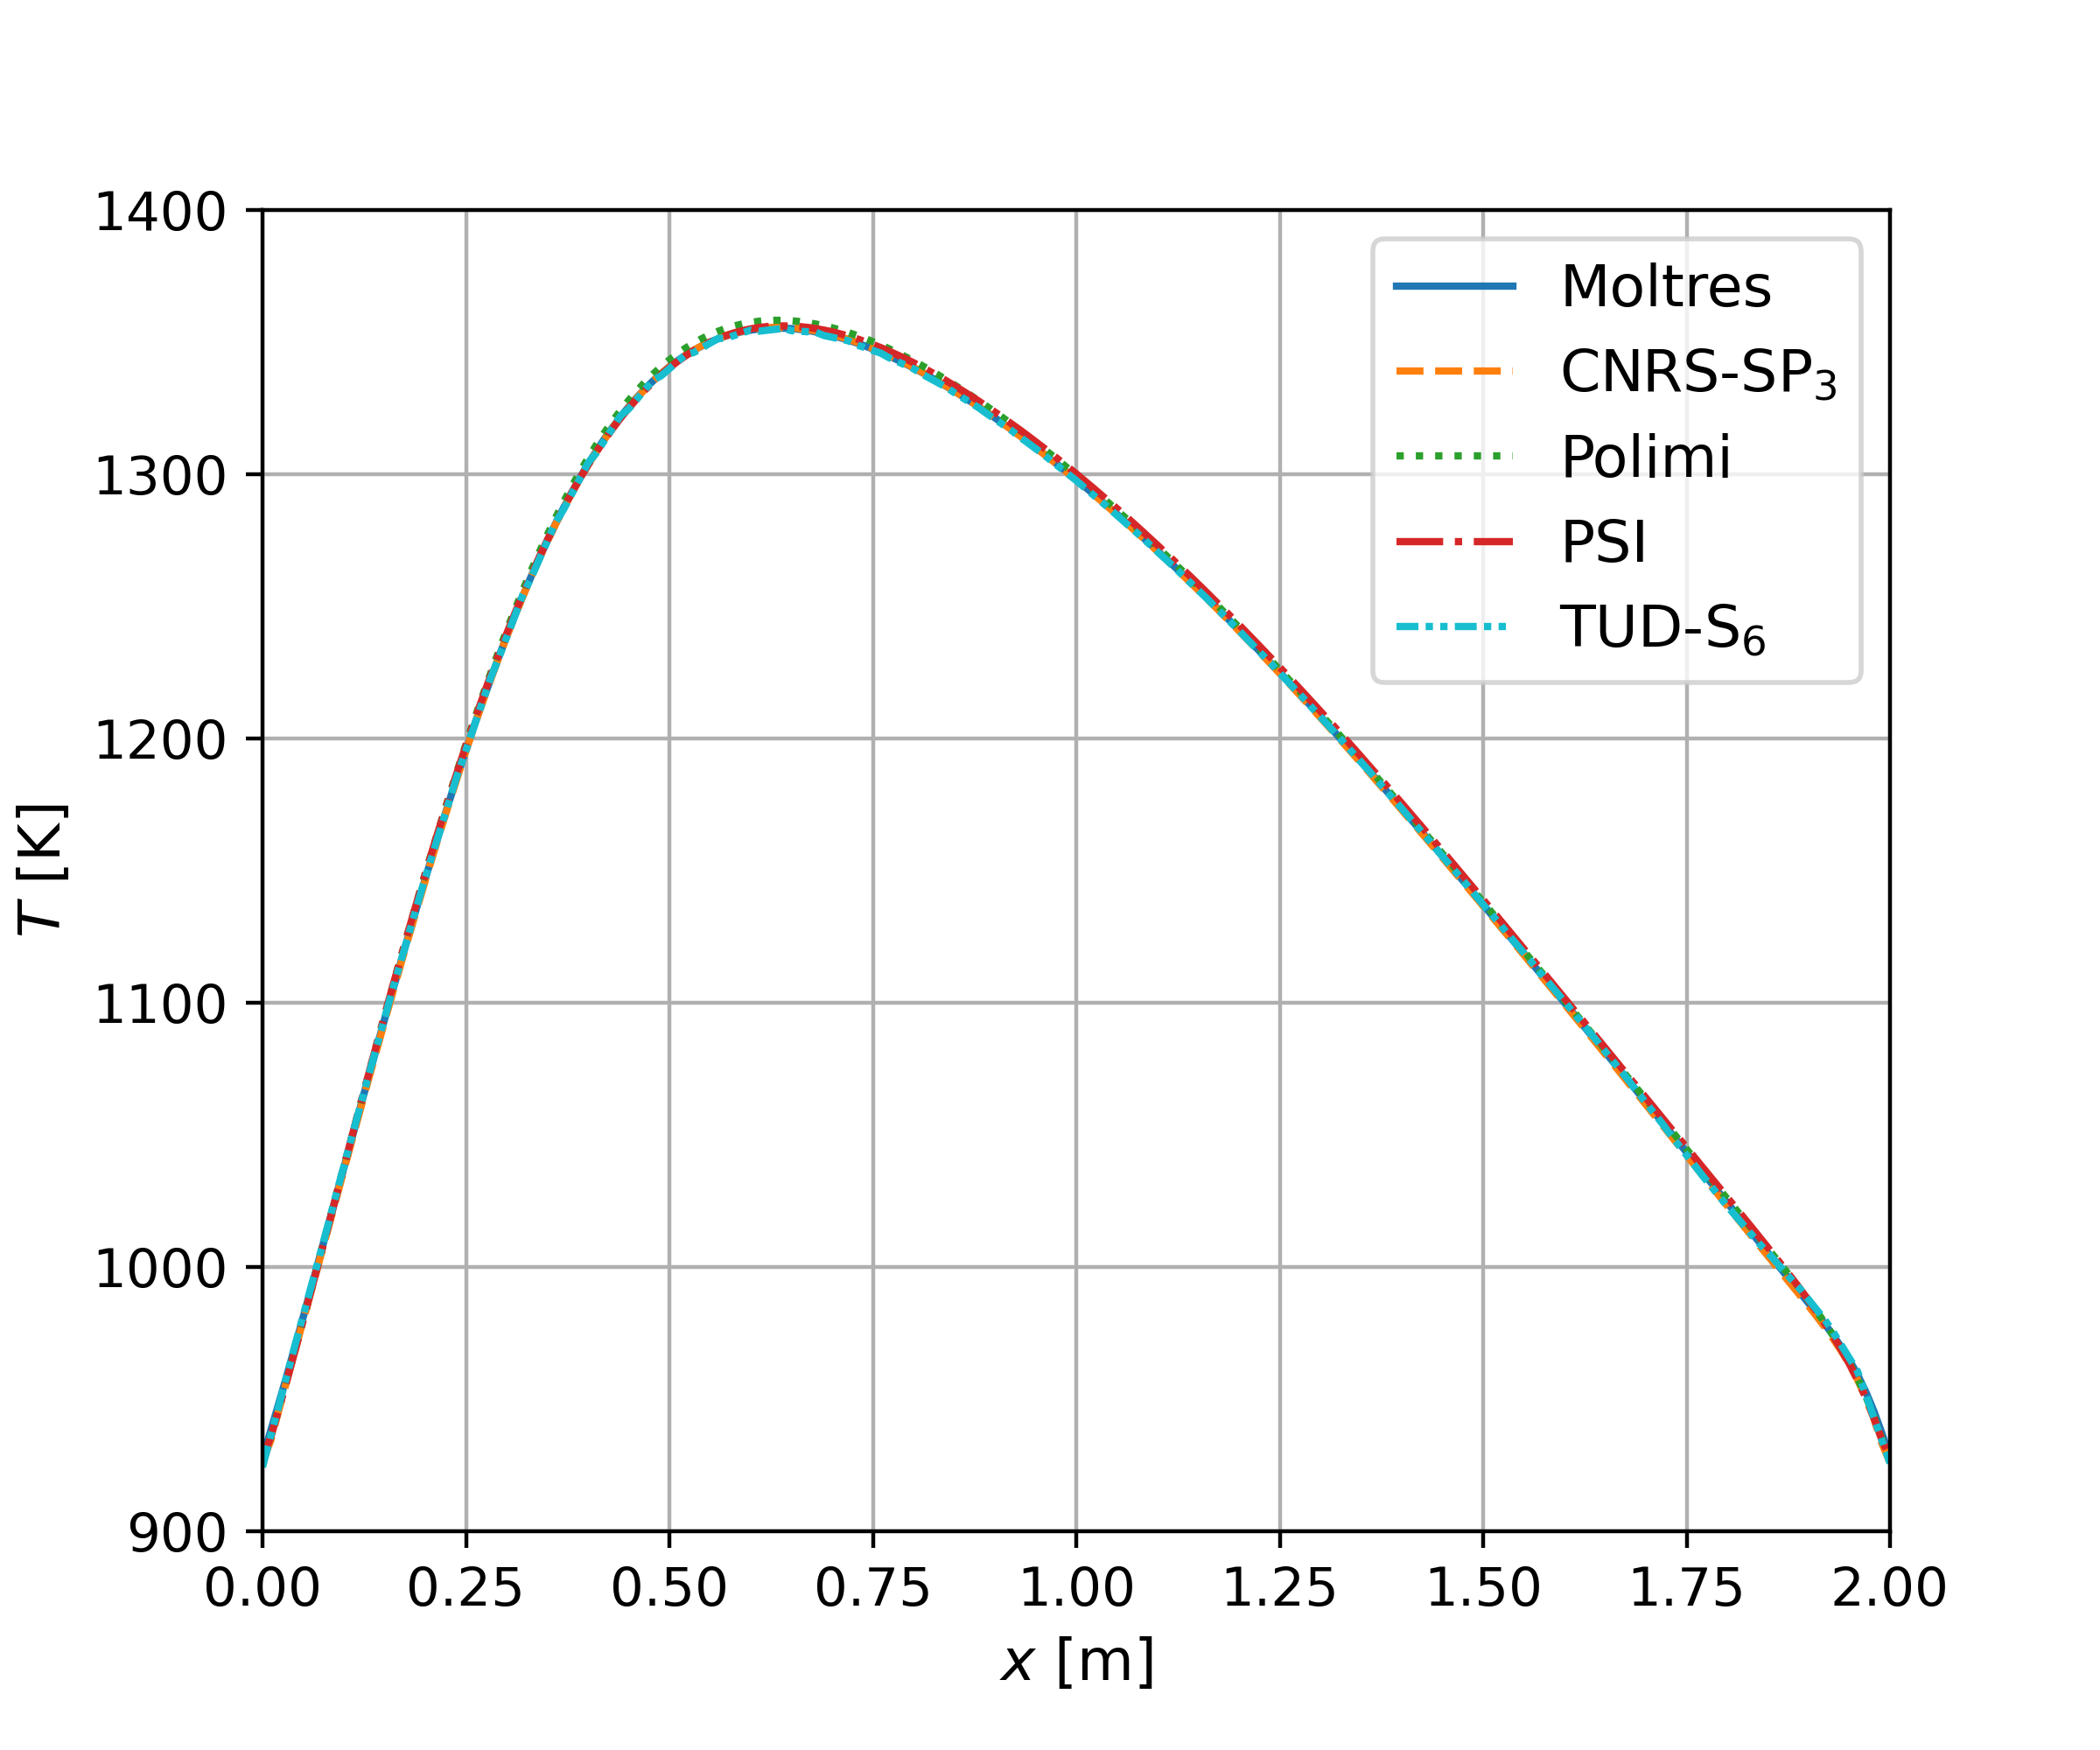
\includegraphics[width=.8\columnwidth]{1-2-temp-plot}
	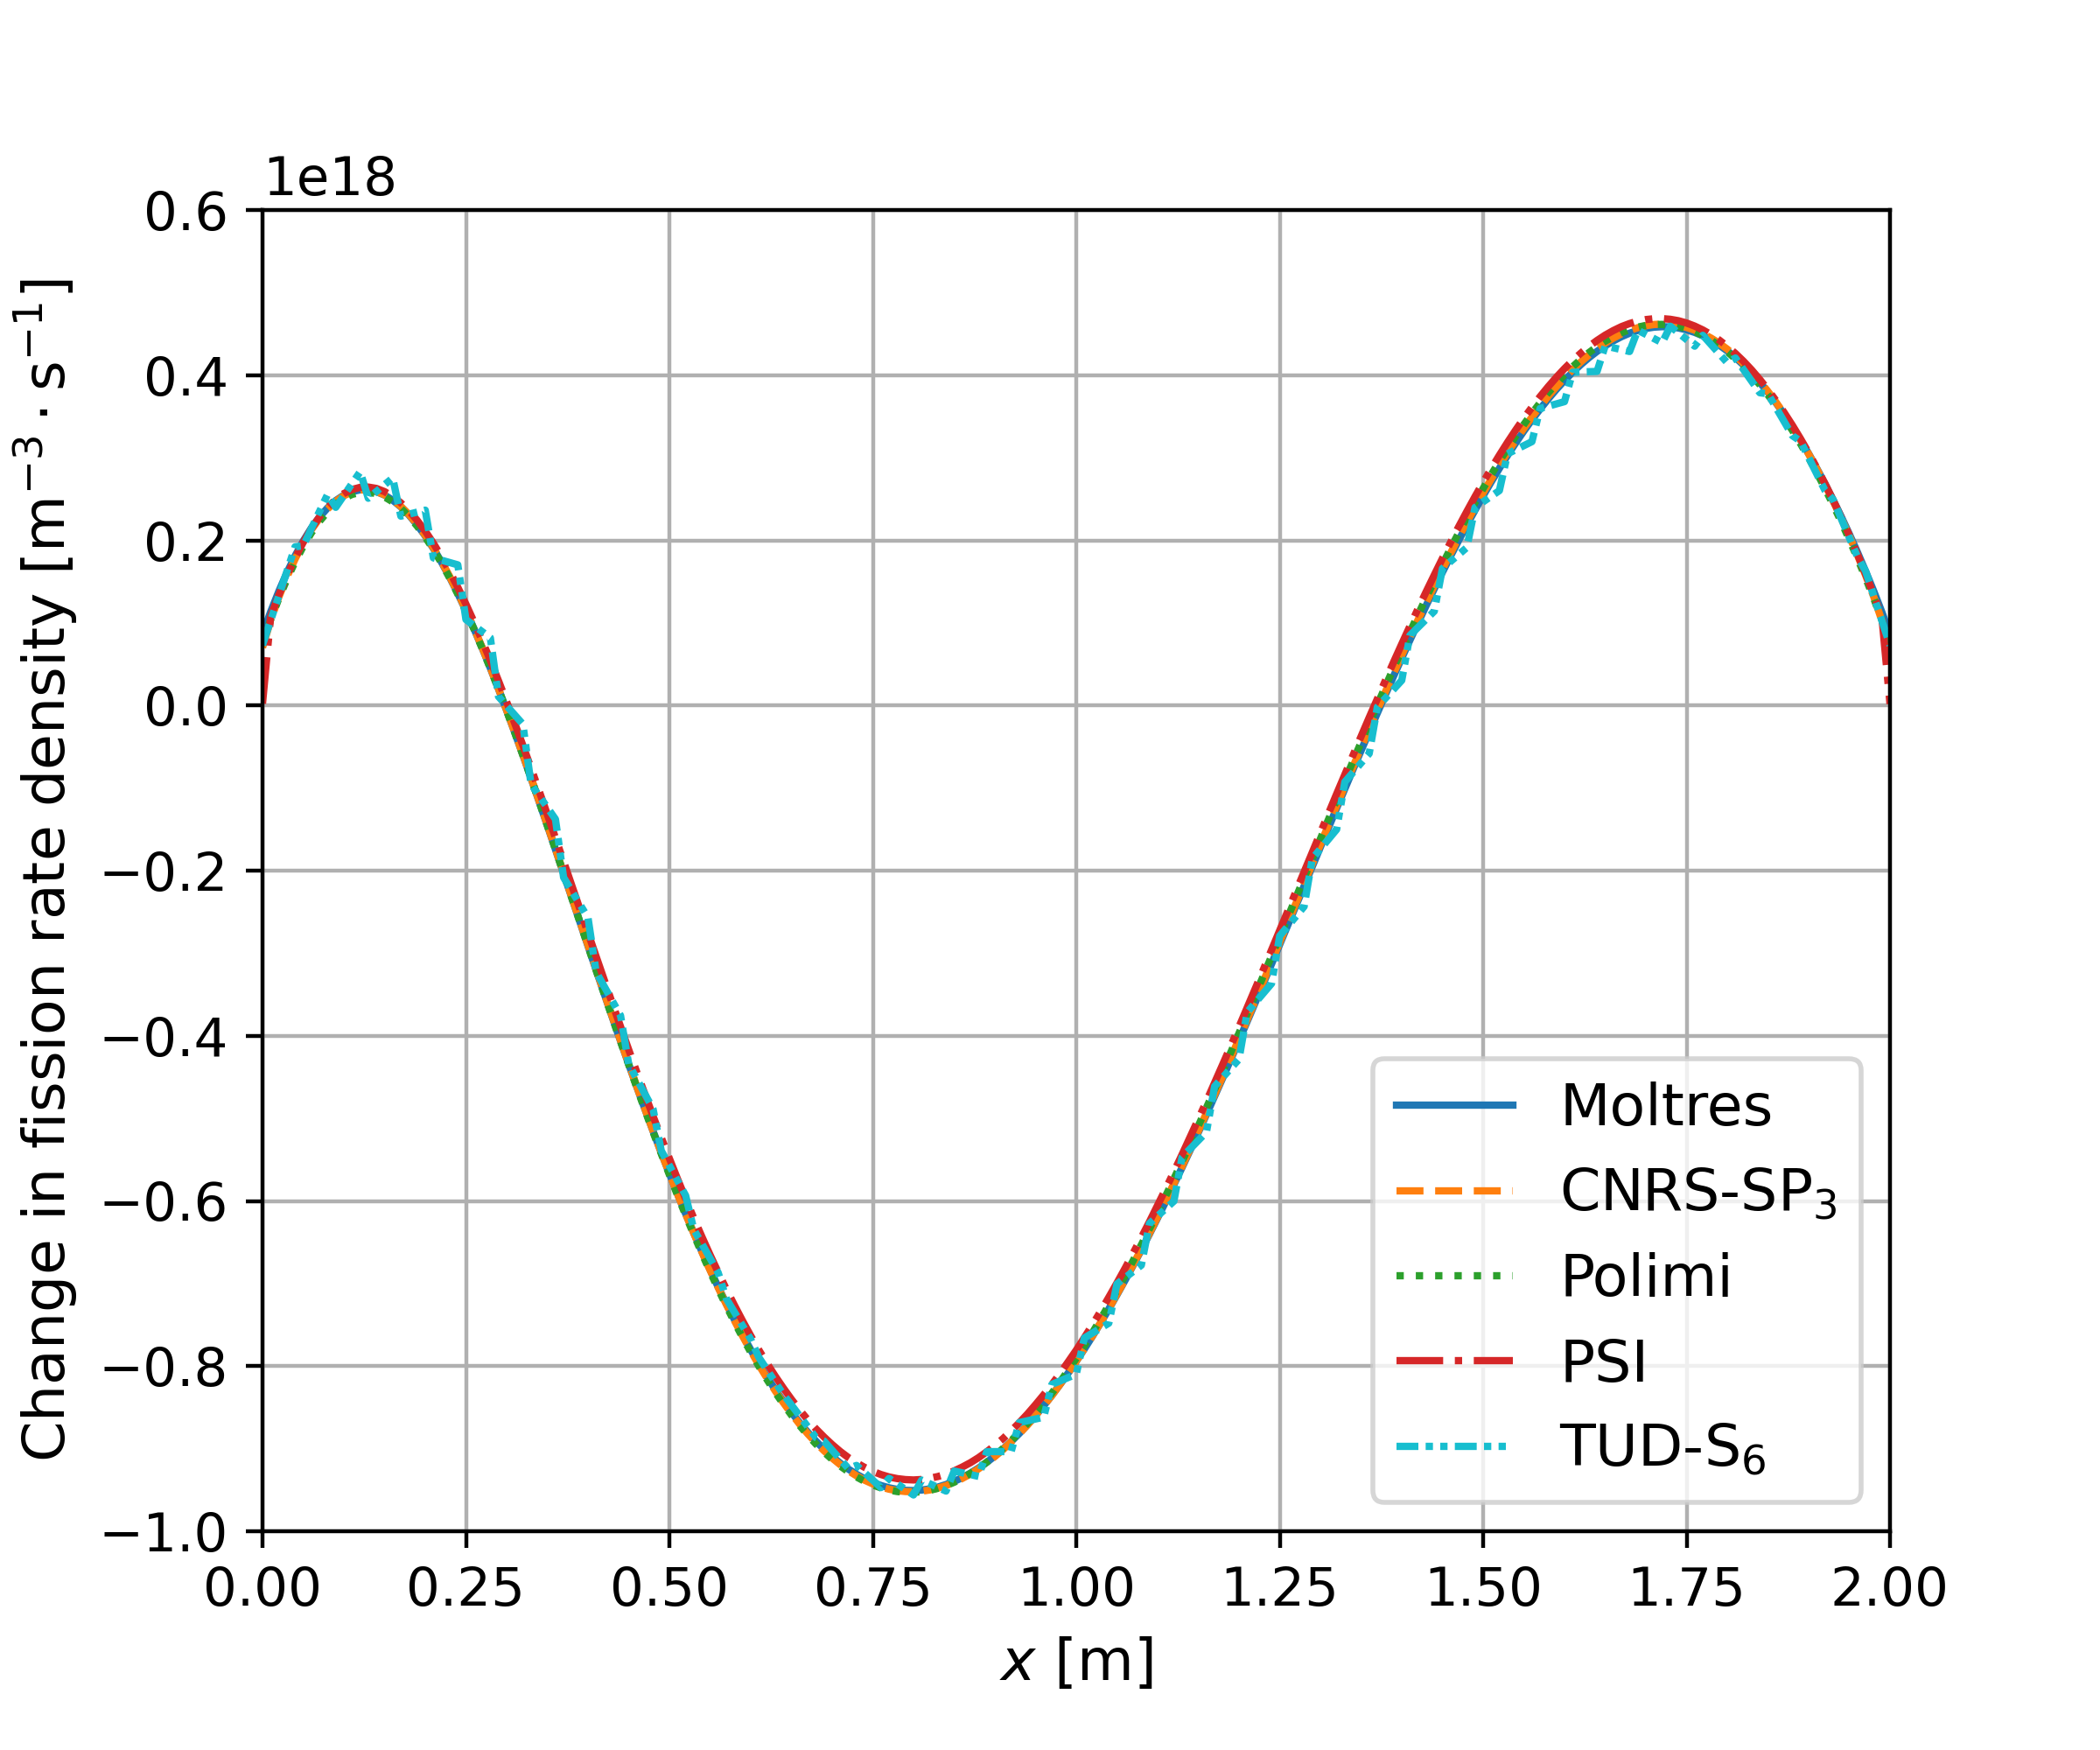
\includegraphics[width=.8\columnwidth]{1-2-fiss-plot}
	\caption{Step 1.2 - Temperature distribution and change in fission rate
	density along AA'.}
	\label{fig:1.2}
\end{figure*}

\subsubsection{Step 1.2: Power coupling}

Figure \ref{fig:1.2} shows the temperature distribution and the change in
fission rate density along AA' from Step 1.2. Similar to Step 0.3, the
temperature distribution from Moltres agrees closest with CNRS-$SP_3$ and
TUD-$S_2$. Table \ref{table:disc1} reports the same trends we observed in Phase
0; the average discrepancy in temperature along BB' from Moltres for Step 1.2
is marginally higher than the benchmark while the average discrepancy in the
fission rate density is on the same order of magnitude as the benchmark.
From Table \ref{table:rho}, Moltres also reports a change in $\rho$
relative to Step 1.1 of $-1142.2$ pcm, that, similar to Steps 0.2 and 1.1,
falls within the range of reported benchmark values.

\subsubsection{Step 1.3: Buoyancy}

Figure \ref{fig:1.3} shows the vertical velocity component, temperature, and
delayed neutron source distributions along AA. As with all previous plots,
Moltres reproduces the correct trend in all three physical
parameters. Step 1.3 has a relatively slower buoyancy-driven flow profile with
no forced flow from the top boundary. Consequently, there are no temperature
deviations near the top boundary and we observe in Table \ref{table:disc1} that
the average discrepancy value of 0.070\% for the temperature distribution along
BB' is much closer to the benchmark value of 0.080\% compared to the
corresponding discrepancy values for Step 0.3 and 1.2.

In Table \ref{table:rho}, we observe that the change in $\rho$ in
Moltres (-1207.7 pcm) falls within the range of reported benchmark values and
matches the software from TUD-$S_2$ (-1208.5 pcm) the closest.
%
\begin{figure*}[tb]
	\centering
	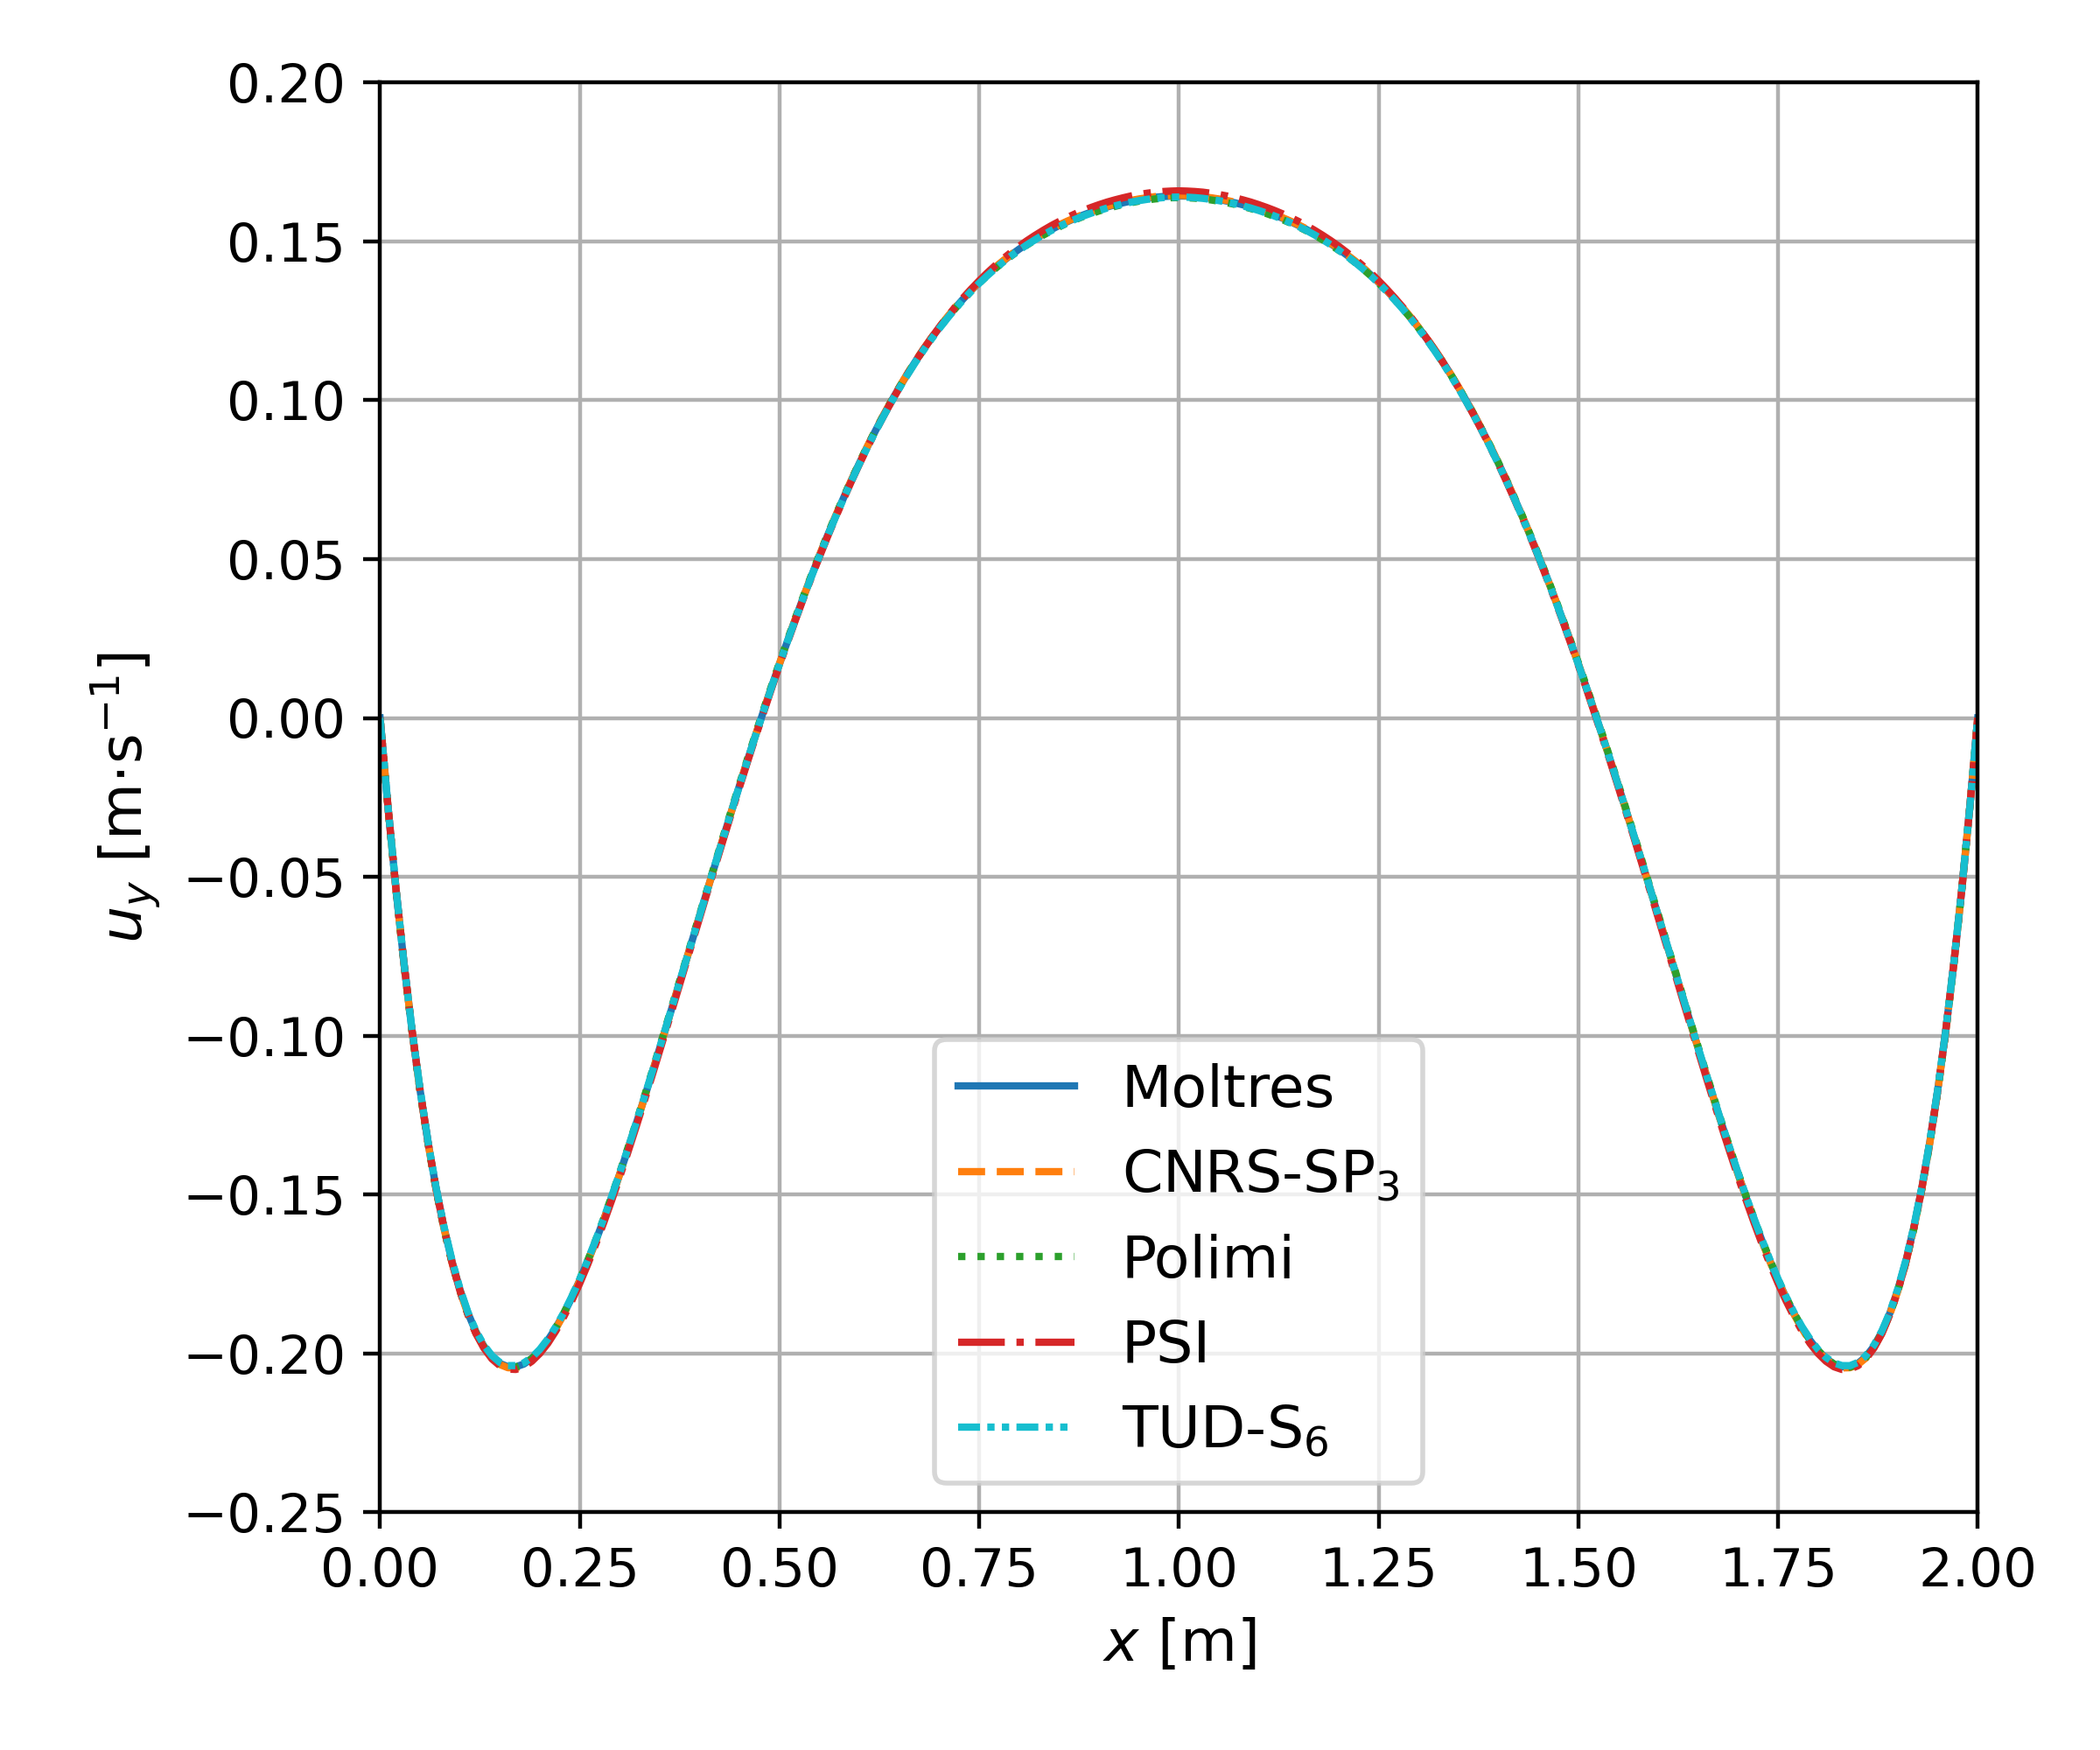
\includegraphics[width=.64\columnwidth]{1-3-vel-plot}
	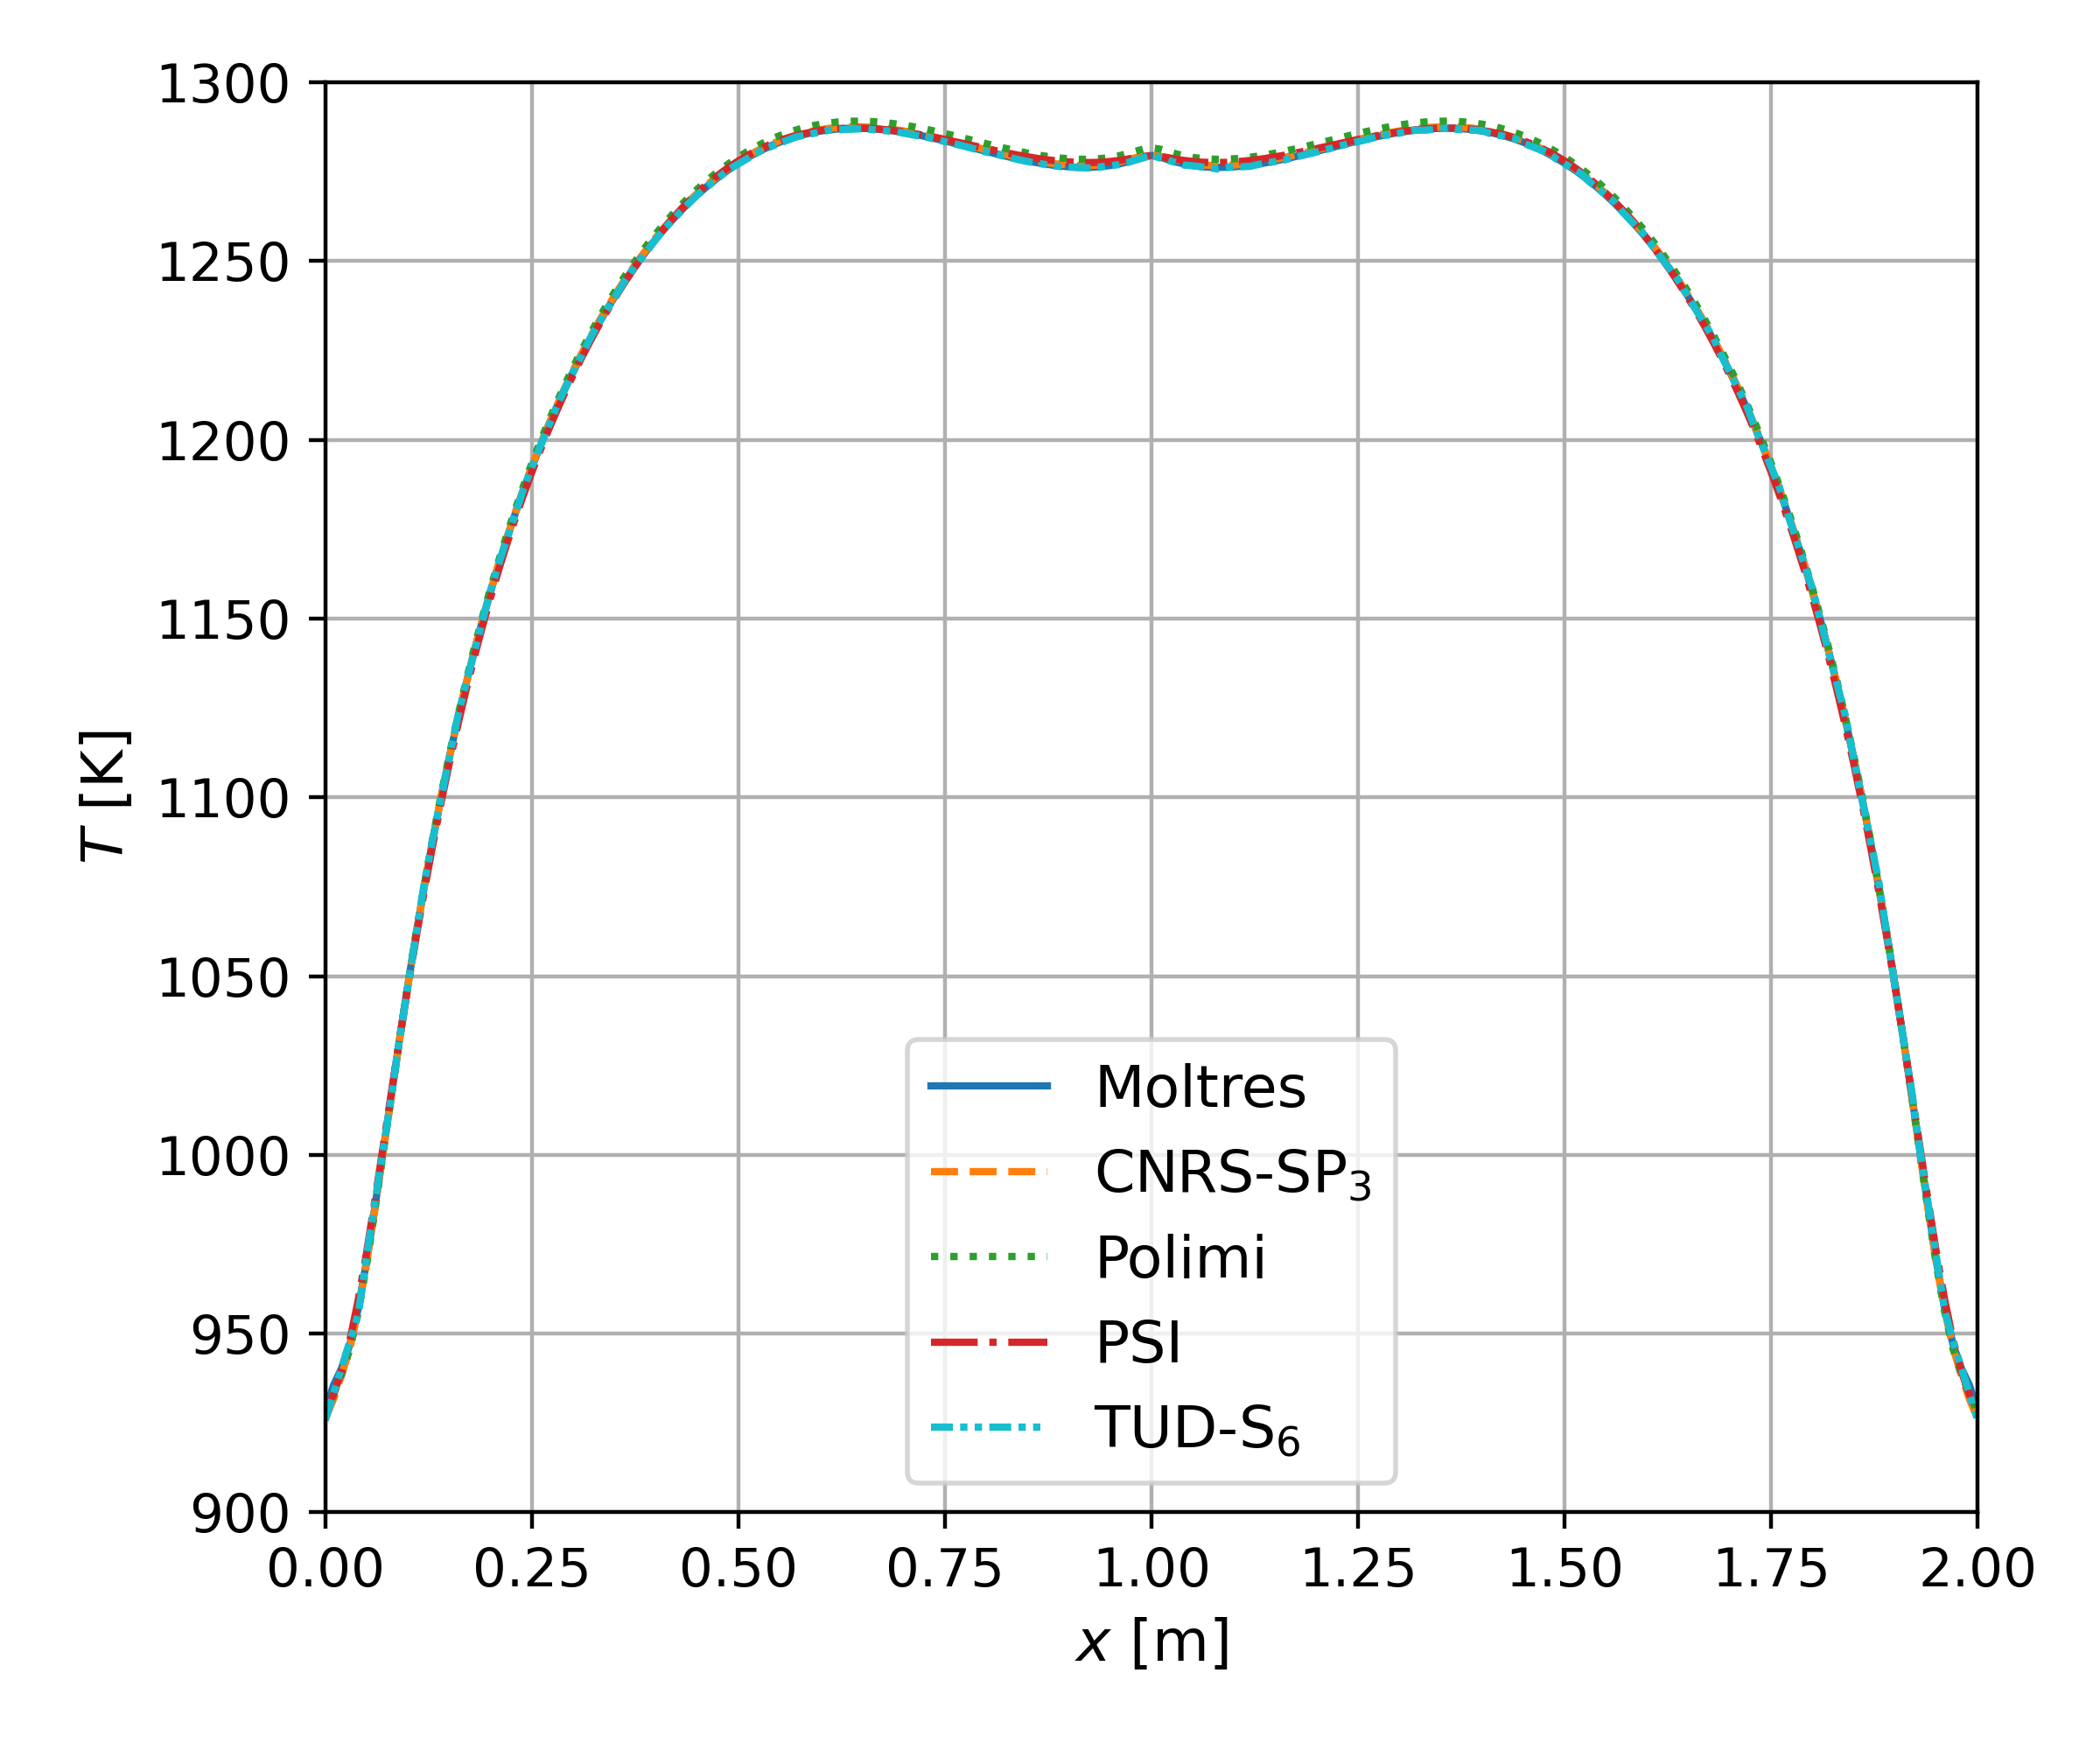
\includegraphics[width=.67\columnwidth]{1-3-temp-plot}
	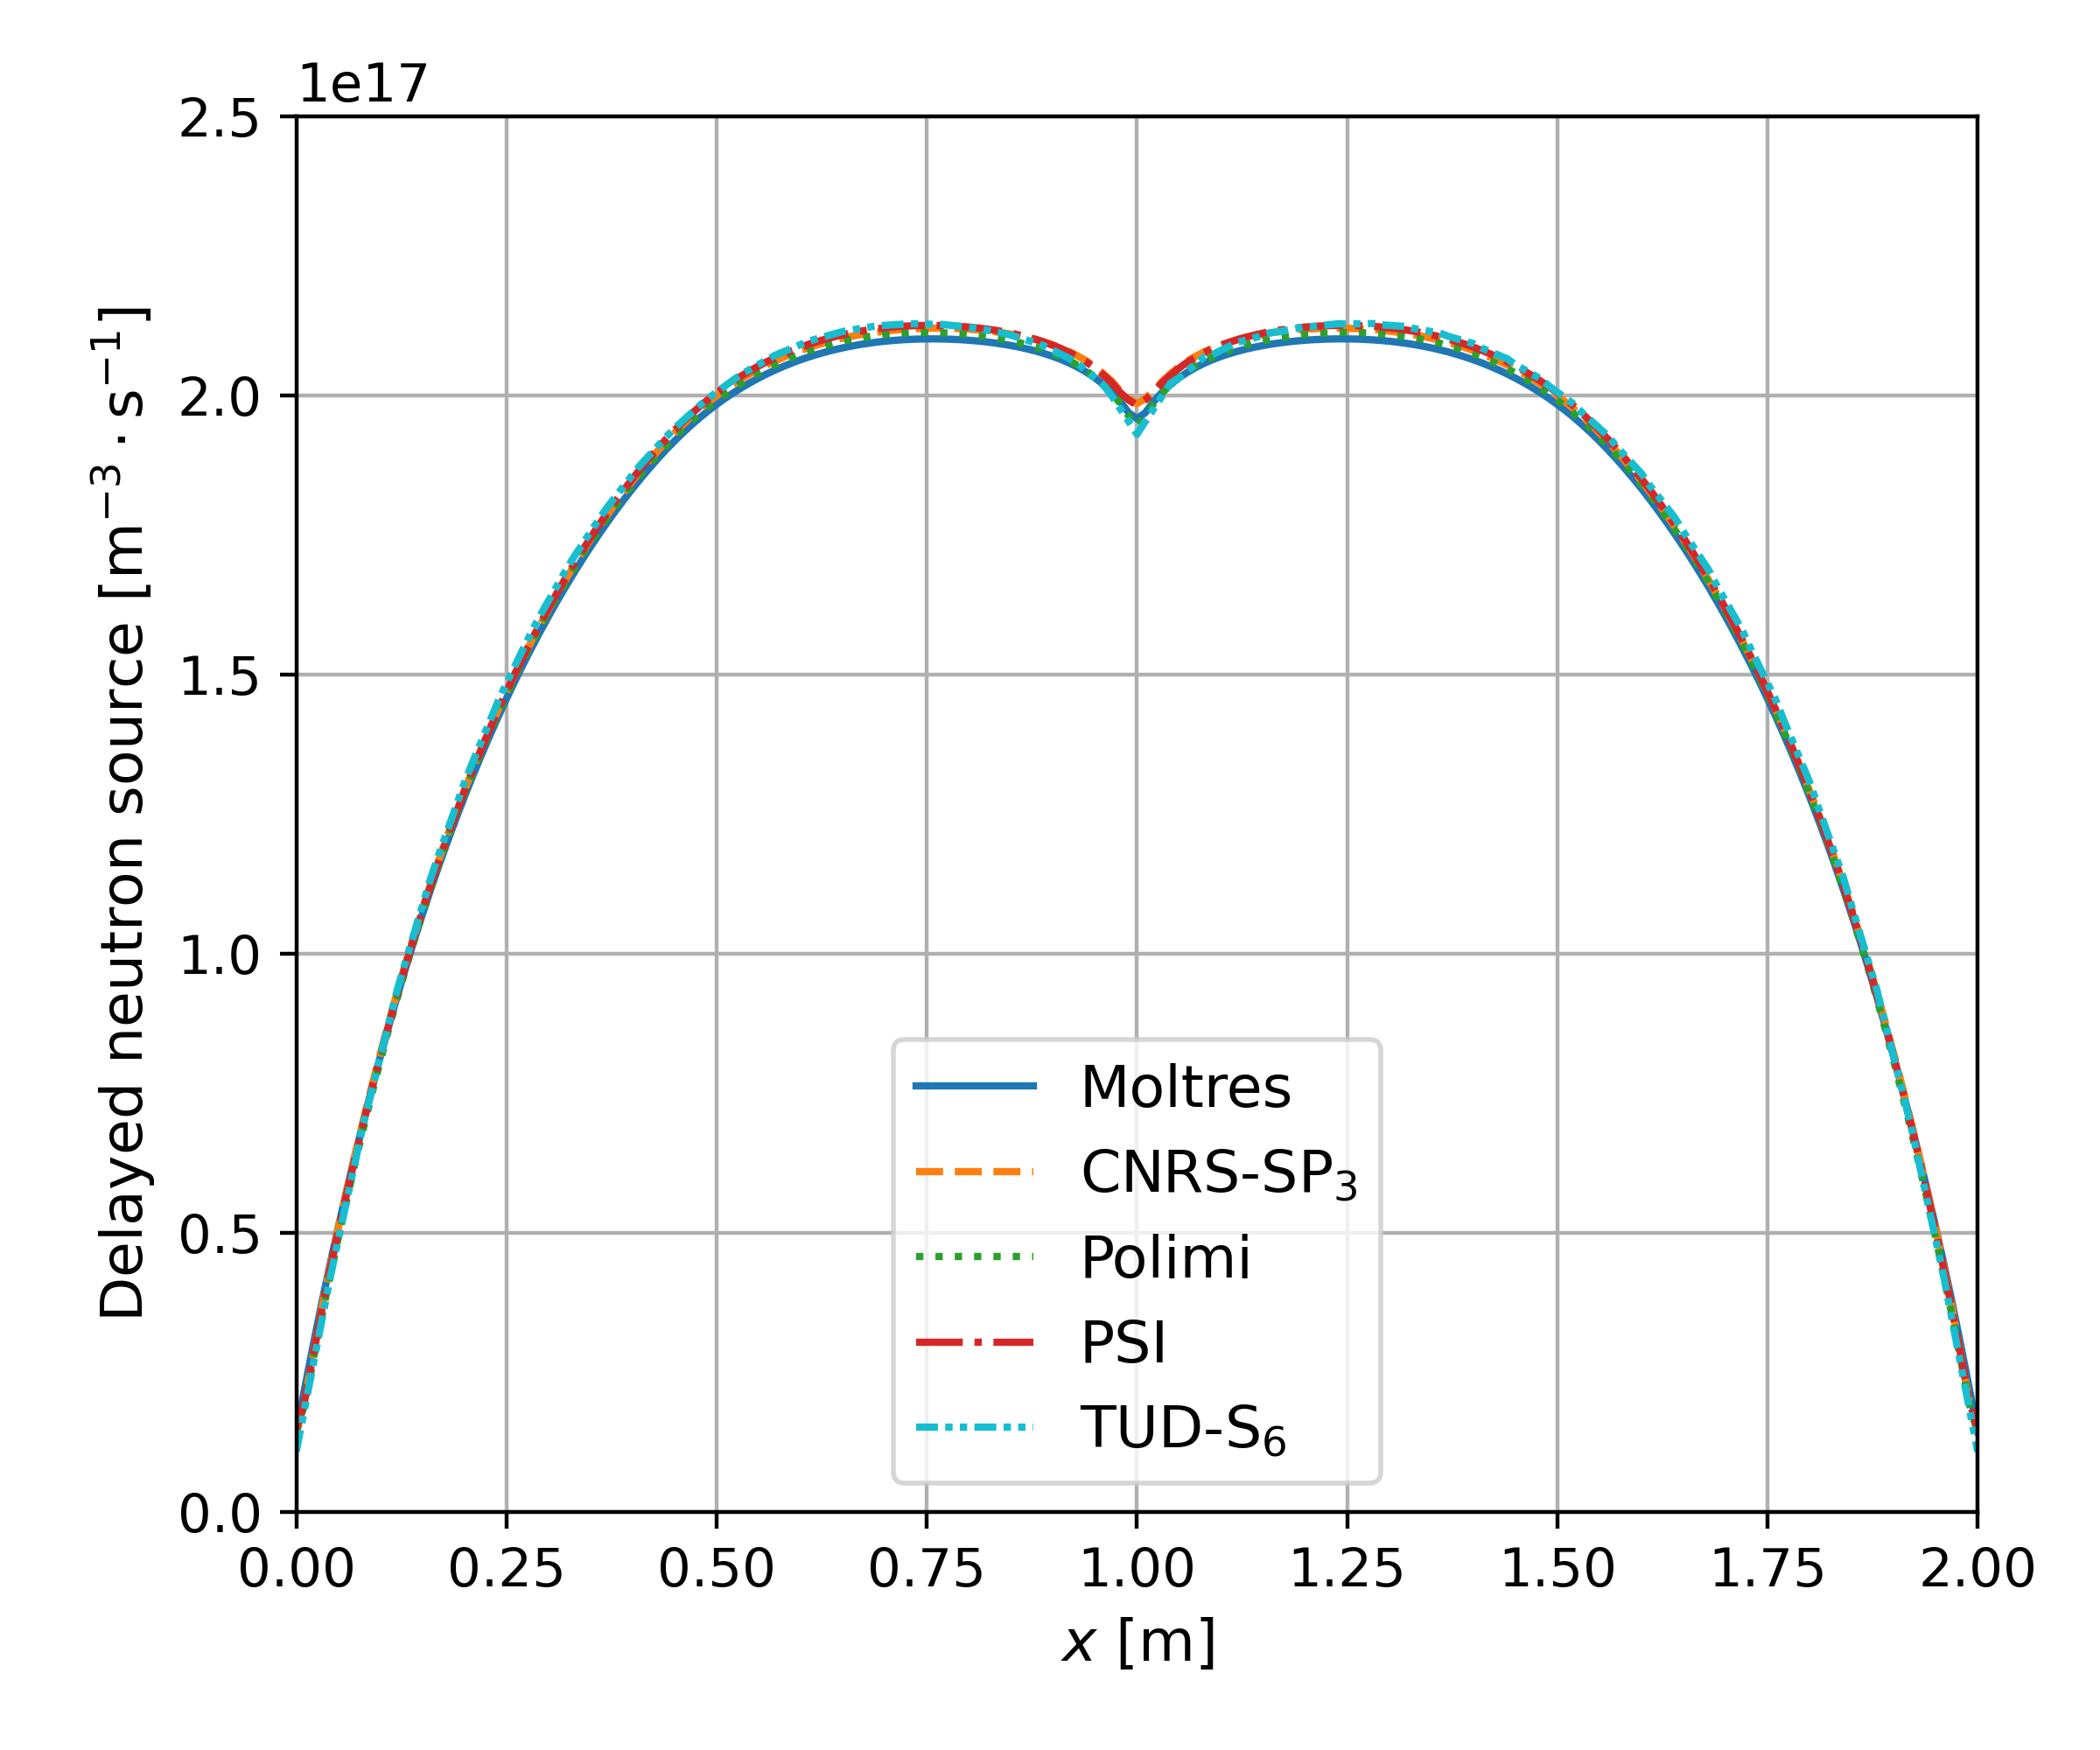
\includegraphics[width=.67\columnwidth]{1-3-dnp-plot}
	\caption{Step 1.3 - Vertical velocity component, temperature distribution,
	and delayed neutron source along AA'.}
	\label{fig:1.3}
\end{figure*}

\subsubsection{Step 1.4: Full coupling}

Figure \ref{fig:color} shows the 2D temperature distribution and velocity
streamlines from Step 1.4 with $U_{lid} = 0.5$ m$\cdot$s$^{-1}$ and $P = 1$ GW.
Table \ref{table:full} shows the change in $\rho$ under the various $U_{lid}$
and $P$ values. We refer readers to Tiberga et al.'s paper
\citep{tiberga_results_2020} for the benchmark's corresponding values.
The results from Moltres all fall within the range of benchmark values for all
cases. Furthermore, the $\Delta\rho$ values are all within 1.1 pcm of the
corresponding values from the TUD-S$_2$ model in the benchmark paper. Given
that the $S_2$ discrete ordinates method is theoretically equivalent to the
multigroup neutron diffusion method, this indicates that Moltres is
consistent with the benchmark outside of differences from the neutronics
models.

\begin{figure}[tb]
  \centering
  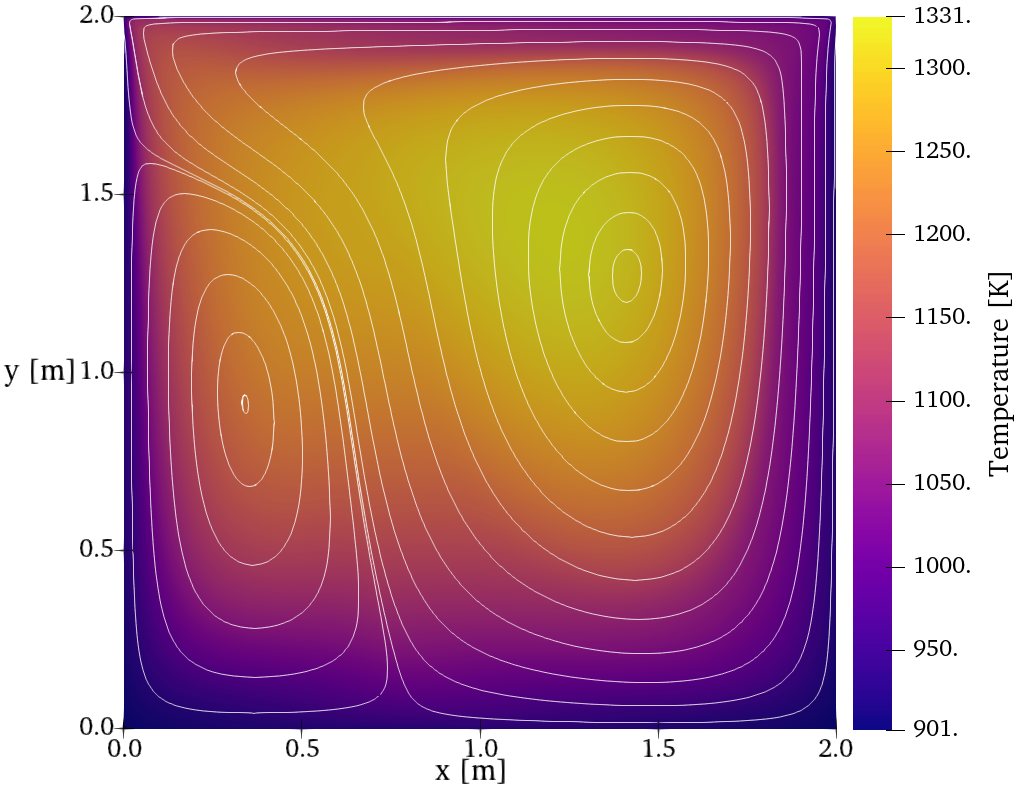
\includegraphics[width=\columnwidth]{full-coupled}
  \caption{The temperature distribution in the domain for the fully coupled
  system (Step 1.4) with buoyancy effects, $P = 1$ GW, and $U_{lid} = 0.5$
  m$\cdot$s$^{-1}$. The lines correspond to the streamlines of the velocity
  field.}
  \label{fig:color}
\end{figure}
%
\begin{table}[tb]
	\caption{Reactivity change in Step 1.4, relative to Step 0.2 under various
	$U_{lid}$ and $P$ values.}
	\centering
	\footnotesize
	\setlength\tabcolsep{1.5pt}
	\begin{tabular}{c c c c c c}
		\toprule
		& \multicolumn{5}{c}{$\rho - \rho_{s0.2}$ [pcm]} \\
		\midrule
		{\backslashbox{$U_{lid}$ [m$\cdot$s$^{-1}$]}{$P$ [GW]}} & 0.2 & 0.4 & 0.6 & 0.8 & 1.0 \\
		\midrule
		0.0 & -263.7 & -498.3 & -730.9 & -966.7 & -1207.7 \\
		0.1 & -265.9 & -498.7 & -730.6 & -966.0 & -1206.7 \\
		0.2 & -268.1 & -498.8 & -729.4 & -963.7 & -1203.6 \\
		0.3 & -269.9 & -498.5 & -727.8 & -960.8 & -1199.5 \\
		0.4 & -271.9 & -498.5 & -726.5 & -958.3 & -1195.7 \\
		0.5 & -274.2 & -498.7 & -725.6 & -956.4 & -1192.7 \\
		\bottomrule
	\end{tabular}
	\label{table:full}
\end{table}
%
\begin{table}[tb]
	\caption{Discrepancy values for the results from Step 2.1.}
	\centering
	\footnotesize
	\begin{tabular}{l l S S}
		\toprule
		\multirow{2}{*}{\textbf{Step}} & \multirow{2}{*}{\textbf{Observable}} & \multicolumn{2}{c}{\textbf{Discrepancies [\%]}} \\
		& & {Moltres} & {Benchmark} \\
		\midrule
		\multirow{2}{*}{2.1} & Gain & 0.496 & 0.587 \\
		\cmidrule{2-4}
		& Phase shift & 1.741 & 2.176\\
		\bottomrule
	\end{tabular}
	\label{table:disc2}
\end{table}
%
\begin{figure*}[tb]
	\centering
	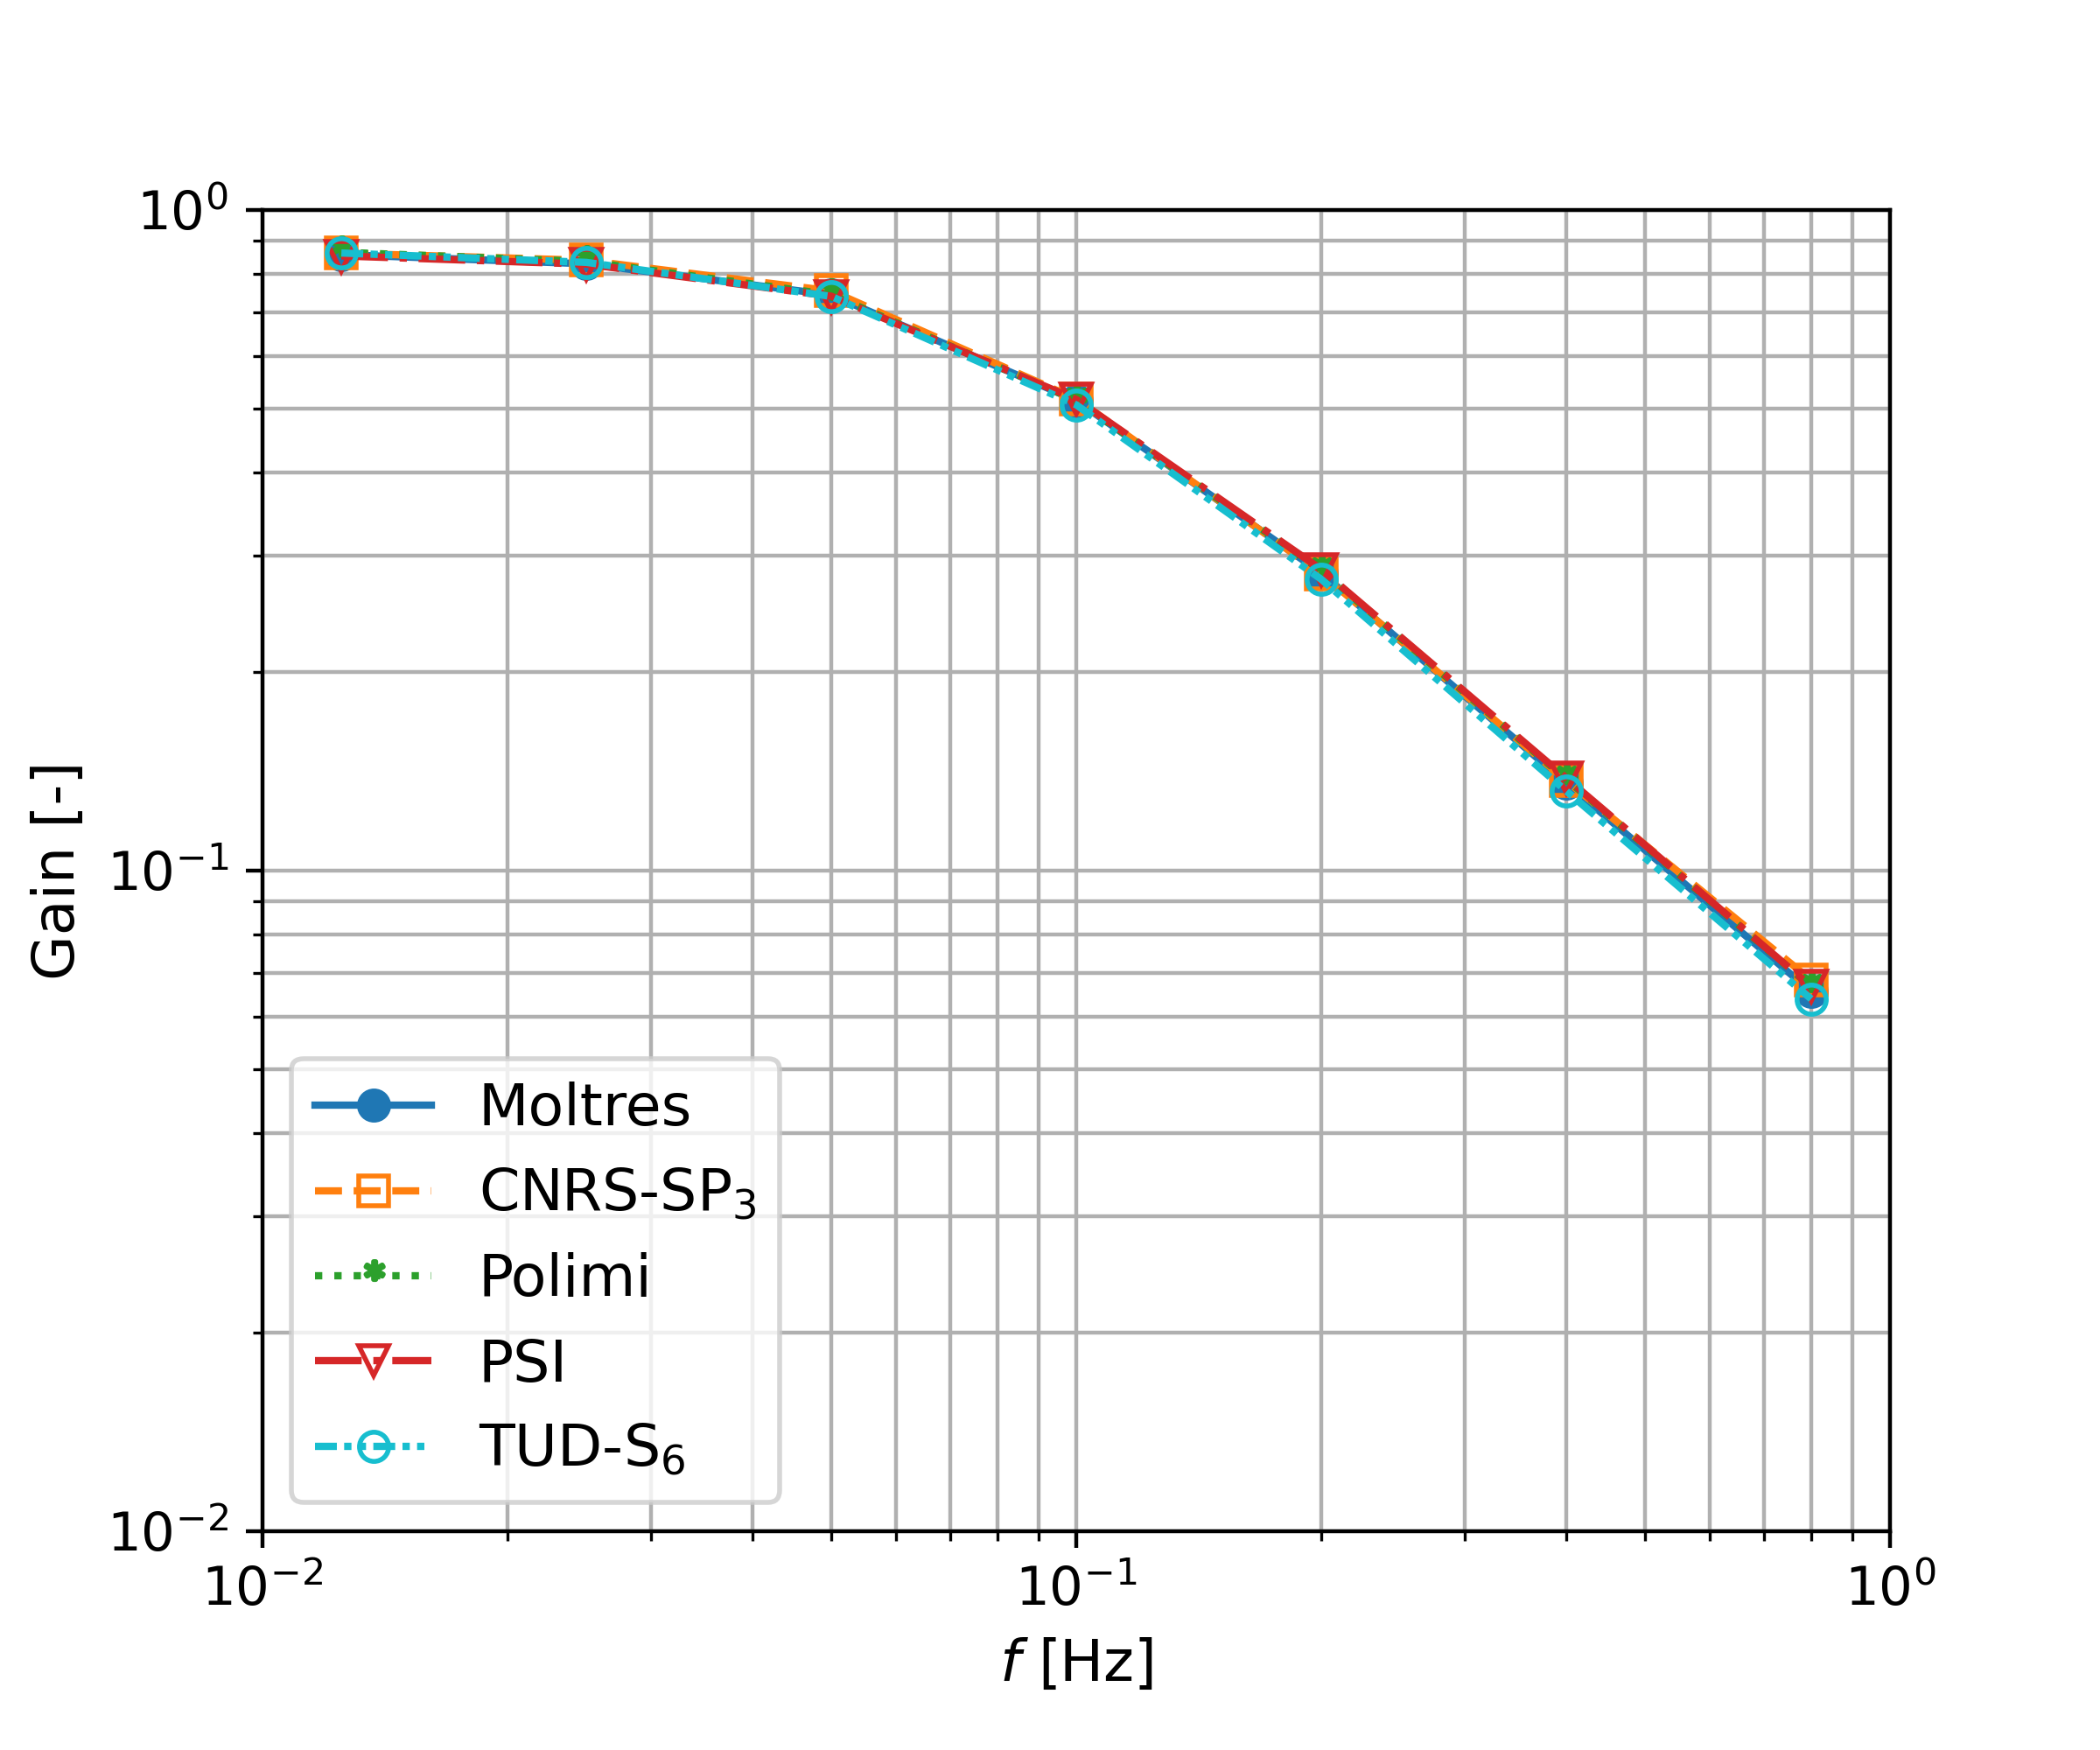
\includegraphics[width=.8\columnwidth]{2-1-gain-plot}
	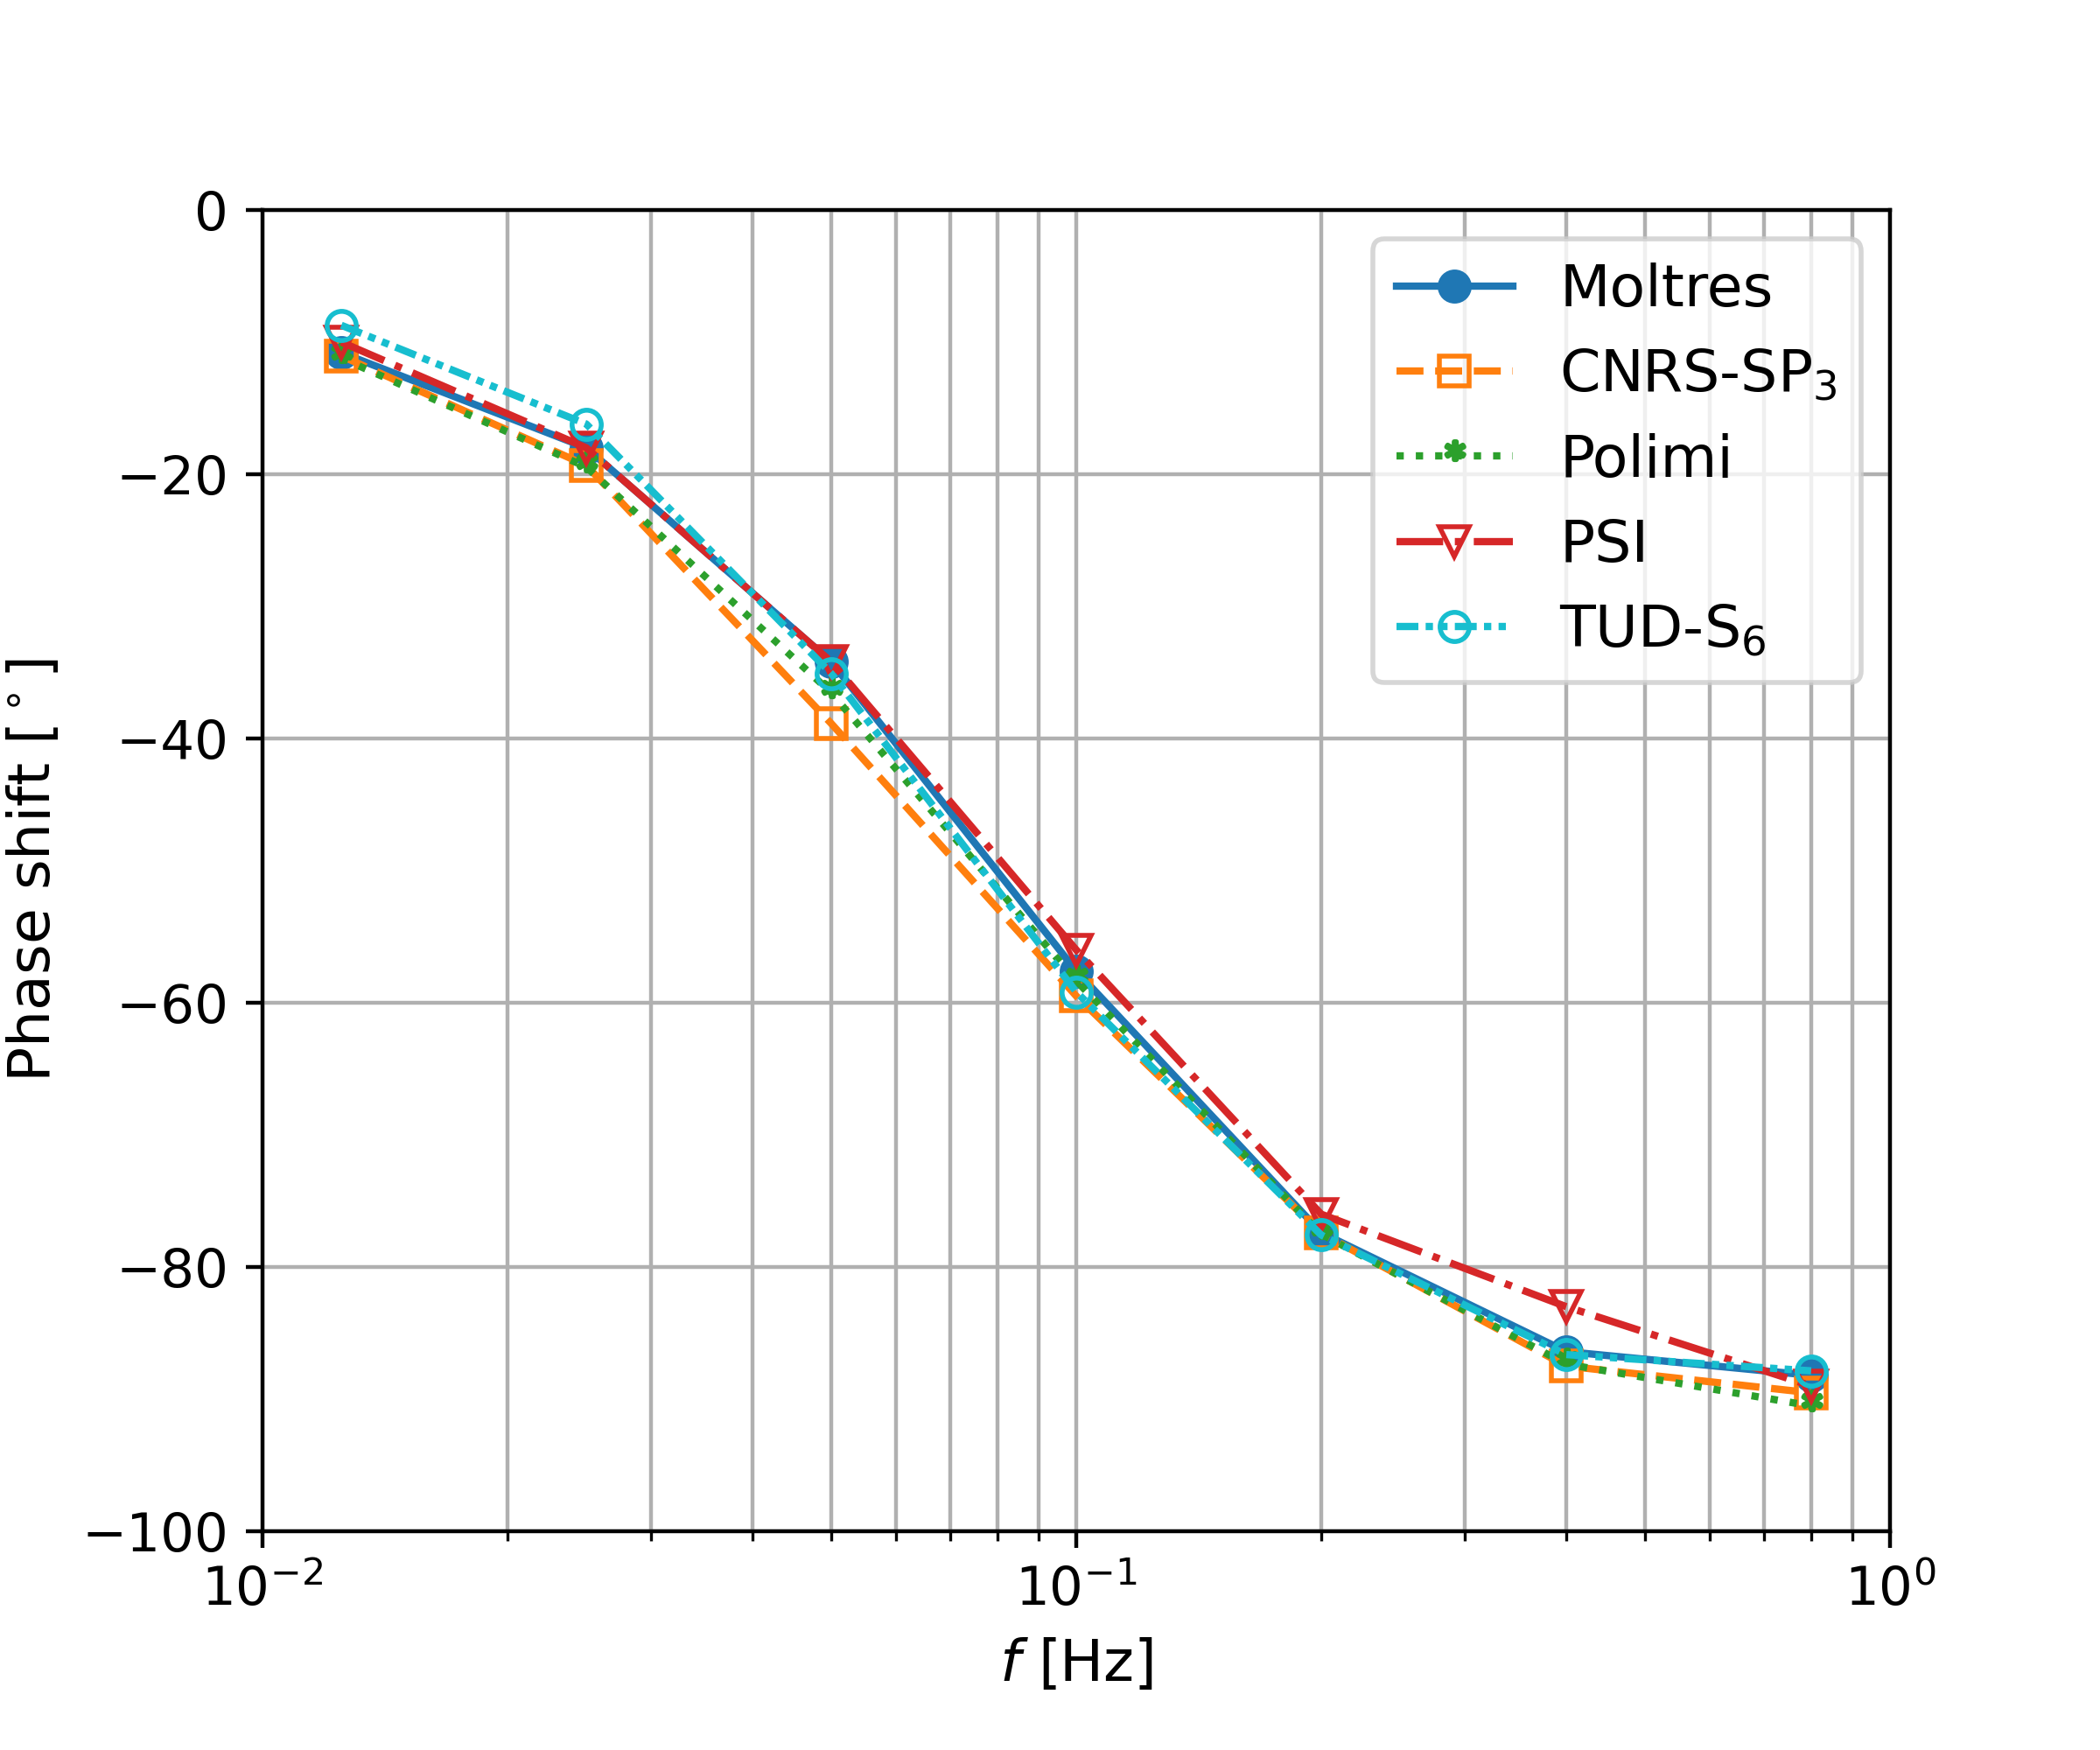
\includegraphics[width=.8\columnwidth]{2-1-phase-plot}
	\caption{Step 2.1 - Bode gain and phase plots of the frequency response of
	the fully coupled system.}
	\label{fig:2.1}
\end{figure*}

\subsection{Phase 2 results \& discussion}

%Transient analysis represents a challenging, yet essential, part of reactor
%safety analysis. A reactor has different timescales for different physical
%phenomena; prompt neutron lifetimes are on the order of microseconds
%while advective heat transfer is relevant in timescales on the order of
%seconds. Additionally, the half-lives of delayed neutron precursors vary from
%milliseconds up to tens of seconds. Obtaining accurate solutions requires tight
%coupling between the neutronics and thermal-hydraulics to adequately capture
%the strong interactions between them and a sufficiently small timestep to
%minimize time discretization errors. The following subsection discusses the
%results from the Step 2.1 transient problem.

\subsubsection{Step 2.1: Forced convection transient}

Figure \ref{fig:2.1} shows the Bode gain and phase shift plots of the response
in power output in the fully coupled system. Along with the average discrepancy
values from Table \ref{table:disc2}, the results show that Moltres is
consistent with the benchmark. The gain data points from all \gls{MSR} software
agree closely with one another. Moltres reports an average discrepancy value of
0.496\%, slightly lower than the benchmark average of 0.587\%. On the other
hand, the phase shift data points show greater spread over the various driving
frequencies. We ascribe this to the different timestepping schemes and timestep
sizes among the different software packages. Even with a precision of
$\pm0.9^\circ$ for each phase shift value, Moltres accurately reproduces the
correct trend with a lower average discrepancy (1.741\%) than the benchmark
average (2.176\%).
